% Marked comparison: unchanged Digest_v1.tex -> main.tex.
% One-column REVIEW layout accommodates original wide digest tables.
% Compile main.tex for the clean six-page conference manuscript.
% Additions have a blue underline; deletions have a red strikethrough for printing.
% The schema has word-level changes; changed table cells are marked individually.
% Replaced comparison/new analysis tables are marked as whole blocks.
% Review graphics are bounded in size; the clean main.tex is unchanged.
%DIF 1-45c1-7
%DIF LATEXDIFF DIFFERENCE FILE
%DIF DEL /tmp/apec-diff-mh2gf9x8/old.tex   Tue Nov 17 11:15:35 2026
%DIF ADD /tmp/apec-diff-mh2gf9x8/new.tex   Tue Nov 17 11:15:35 2026
%DIF < \documentclass[conference,onecolumn,letterpaper,romanappendices,12pt,english,nofonttune]{IEEEtran}
%DIF <     \IEEEoverridecommandlockouts
%DIF < \usepackage[margin=1in]{geometry}
%DIF < \usepackage{setspace}
%DIF < \usepackage{tablefootnote}
%DIF < \usepackage[compact]{titlesec}
%DIF < \usepackage{float}
%DIF <     \titlespacing{\title}{0pt}{0pt}{24pt}
%DIF <     \titlespacing{\section}{0pt}{10pt}{6pt}
%DIF <     \titlespacing{\subsection}{0pt}{*0}{*0}
%DIF <     \titlespacing{\subsubsection}{0pt}{*0}{*0}
%DIF <     \titlespacing{\appendix}{0pt}{*0}{*0}
%DIF <
%DIF <
%DIF < \renewcommand{\appendix}{}
%DIF <
%DIF < \usepackage[runin]{abstract}
%DIF <     \renewcommand{\abstractnamefont}{\normalfont\normalsize\itshape}
%DIF <     \renewcommand{\abstracttextfont}{\normalfont\normalsize}
%DIF <     \setlength{\absleftindent}{0mm}
%DIF <     \setlength{\absrightindent}{0mm}
%DIF <     \abslabeldelim{--}
%DIF <
%DIF < \usepackage{lastpage}
%DIF < \usepackage{fancyhdr}
%DIF <     \setlength{\headheight}{0.6in}
%DIF <     \setlength{\headsep}{15pt}
%DIF <     \setlength{\voffset}{-0.5in}
%DIF <     \renewcommand{\headrulewidth}{0pt} % remove lines as well
%DIF <     \renewcommand{\footrulewidth}{0pt}
%DIF <     \fancyhf{}
%DIF <     \fancyfoot[C]{\thepage\ of \pageref{LastPage}}
%DIF <     \pagestyle{fancy}
%DIF <
%DIF < \usepackage[ngerman,main=english]{babel}
%DIF < \usepackage{xcolor}
%DIF < \usepackage[pdftex]{graphicx}
%DIF < \usepackage{wrapfig}
%DIF < \usepackage{newtxtext,newtxmath}
%DIF < \usepackage[group-minimum-digits=4,per-mode=fraction]{siunitx}
%DIF < \usepackage[T1]{fontenc}
%DIF < \usepackage{caption}
%DIF < 	\captionsetup[table]{labelsep=period,font=small,font=sc}
%DIF < 	\captionsetup[figure]{font=small,justification=centerlast}
%DIF < \usepackage{subcaption}
%DIF -------
\RequirePackage[T1]{fontenc} %DIF >
\documentclass[conference,onecolumn,letterpaper]{IEEEtran} %DIF >
\usepackage{cite} %DIF >
\usepackage{amsmath,amssymb} %DIF >
\interdisplaylinepenalty=2500 %DIF >
\usepackage{graphicx} %DIF >
\usepackage{array} %DIF >
%DIF -------
\usepackage{booktabs}
%DIF 47-66c9
%DIF <
%DIF < \usepackage{enumitem}
%DIF < \usepackage{soul}
%DIF < \usepackage[noadjust]{cite}
%DIF <
%DIF < \usepackage[capitalize,noabbrev]{cleveref}
%DIF <     \crefname{figure}{Fig.}{Figs.}
%DIF <     \crefname{equation}{}{}
%DIF <     \crefname{section}{Section}{Sections}
%DIF <     \crefname{table}{Table}{Tables}
%DIF <
%DIF < \usepackage{multirow}
%DIF <
%DIF < \renewcommand{\IEEEbibitemsep}{6pt}
%DIF < \makeatletter
%DIF < \IEEEtriggercmd{\reset@font\normalfont\fontsize{12pt}{12pt}\selectfont}
%DIF < \makeatother
%DIF < \IEEEtriggeratref{1}
%DIF <
%DIF < %---folder for graphics and plots
%DIF -------
\usepackage{url} %DIF >
%DIF -------
\graphicspath{{./figures/}}
%DIF 68c11-12
%DIF <
%DIF -------
\setlength{\textfloatsep}{12pt plus 2pt minus 2pt} %DIF >
\setlength{\dbltextfloatsep}{12pt plus 2pt minus 2pt} %DIF >
%DIF -------
\hyphenation{op-tical net-works semi-conduc-tor}
%DIF <
%DIF <
%DIF PREAMBLE EXTENSION ADDED BY LATEXDIFF
%DIF CFONT PREAMBLE %DIF PREAMBLE
\RequirePackage{color}\definecolor{RED}{rgb}{1,0,0}\definecolor{BLUE}{rgb}{0,0,1} %DIF PREAMBLE
\DeclareOldFontCommand{\sf}{\normalfont\sffamily}{\mathsf} %DIF PREAMBLE
\providecommand{\DIFadd}[1]{{\protect\color{blue} \sf #1}} %DIF PREAMBLE
\providecommand{\DIFdel}[1]{{\protect\color{red} \scriptsize #1}} %DIF PREAMBLE
%DIF SAFE PREAMBLE %DIF PREAMBLE
\providecommand{\DIFaddbegin}{} %DIF PREAMBLE
\providecommand{\DIFaddend}{} %DIF PREAMBLE
\providecommand{\DIFdelbegin}{} %DIF PREAMBLE
\providecommand{\DIFdelend}{} %DIF PREAMBLE
\providecommand{\DIFmodbegin}{} %DIF PREAMBLE
\providecommand{\DIFmodend}{} %DIF PREAMBLE
%DIF FLOATSAFE PREAMBLE %DIF PREAMBLE
\providecommand{\DIFaddFL}[1]{\DIFadd{#1}} %DIF PREAMBLE
\providecommand{\DIFdelFL}[1]{\DIFdel{#1}} %DIF PREAMBLE
\providecommand{\DIFaddbeginFL}{} %DIF PREAMBLE
\providecommand{\DIFaddendFL}{} %DIF PREAMBLE
\providecommand{\DIFdelbeginFL}{} %DIF PREAMBLE
\providecommand{\DIFdelendFL}{} %DIF PREAMBLE
%DIF END PREAMBLE EXTENSION ADDED BY LATEXDIFF

\usepackage{float}
\providecommand{\bstctlcite}[1]{}
\usepackage[normalem]{ulem}
\emergencystretch=3em
\renewcommand{\DIFadd}[1]{{\protect\color{blue}\protect\uline{#1}}}
\renewcommand{\DIFdel}[1]{{\protect\color{red}\protect\sout{#1}}}
\newcommand{\APECReviewOldTableA}{%
\begin{table}[H]
    \centering\color{red}
    \caption{\DIFdel{Performance Comparison with Existing Cyber Anomaly Detection Schemes}}
    \label{tab:comparison_digest}
    \renewcommand{\arraystretch}{1.3} % Adds a little padding to the rows
    \begin{tabular}{|l|c|c|c|c|}
        \hline
\DIFdel{\textbf{Methodology}} & \DIFdel{\textbf{Sensor Data}} & \DIFdel{\textbf{Accuracy}} & \DIFdel{\textbf{Real-Time}} & \DIFdel{\textbf{Edge Scalability}} \\
        \hline
\DIFdel{Aljohani \textit{et al.} \mbox{\cite{aljohani2024}} (LSTM)} & \DIFdel{IED / Substation} & \DIFdel{$\sim$95\%} & \DIFdel{Yes} & \DIFdel{Low (High Cost)} \\
        \hline
\DIFdel{Guha \textit{et al.} \mbox{\cite{guha}} (VAE)} & \DIFdel{PMU} & \DIFdel{$\sim$89\%} & \DIFdel{No} & \DIFdel{Low (High Cost)} \\
        \hline
\DIFdel{Initial Baseline (Standard LSTM)} & \DIFdel{EMU} & \DIFdel{$\sim$81\%} & \DIFdel{Yes} & \DIFdel{High (Low Cost)} \\
        \hline
\DIFdel{\textbf{Proposed (Bi-GRU)}} & \DIFdel{\textbf{EMU}} & \DIFdel{\textbf{$\sim$92\%}} & \DIFdel{\textbf{Yes}} & \DIFdel{\textbf{High (Low Cost)}} \\
        \hline
    \end{tabular}
\end{table}
}
\newcommand{\APECReviewNewTableA}{%
\begin{table}[!t]
\centering\color{blue}
\caption{\DIFadd{Comparison with existing electrical anomaly-detection and PCC-monitoring methods. Different datasets and sensing setups were used; the comparison concerns task and sensing scope.}}
\label{tab:prior_work}
\small
\setlength{\tabcolsep}{3pt}
\begin{tabular}{@{}p{.28\linewidth}p{.30\linewidth}p{.35\linewidth}@{}}
\toprule
\DIFadd{Work} & \DIFadd{Sensing/setting} & \DIFadd{Objective} \\
\midrule
\DIFadd{Aljohani et al.~\mbox{\cite{aljohani2024}}} & \DIFadd{IED/substation} & \DIFadd{FDIA detection and mitigation} \\
\DIFadd{Guha et al.~\mbox{\cite{guha}}} & \DIFadd{Grid phasor time series} & \DIFadd{Unsupervised anomaly detection} \\
\DIFadd{Dasari et al.~\mbox{\cite{pmu_lstm_2025}}} & \DIFadd{PMU/IEEE 39-bus} & \DIFadd{Multiclass anomaly detection} \\
\DIFadd{Najar et al.~\mbox{\cite{najarSOC2026}}} & \DIFadd{Smart-plug PCC} & \DIFadd{Battery state-of-charge estimation} \\
\DIFadd{Proposed} & \DIFadd{EMU/two-motor PCC} & \DIFadd{FDIA detection, motor and phase identification} \\
\bottomrule
\end{tabular}
\end{table}
}
\newcommand{\APECReviewNewTableB}{%
\begin{table}[!t]
\centering\color{blue}
\caption{\DIFadd{Binary FDIA detection performance. Rates are percentages; FPR denotes false-positive rate.}}
\label{tab:comparison}
\setlength{\tabcolsep}{3pt}
\small
\begin{tabular}{lrrrr}
\toprule
\DIFadd{Model} & \DIFadd{Accuracy} & \DIFadd{Bal. acc.} & \DIFadd{Recall} & \DIFadd{FPR} \\
\midrule
\DIFadd{LSTM} & \DIFadd{84.89} & \DIFadd{64.15} & \DIFadd{98.33} & \DIFadd{70.04} \\
\DIFadd{CNN--LSTM} & \DIFadd{89.81} & \DIFadd{85.33} & \DIFadd{92.71} & \DIFadd{22.05} \\
\DIFadd{CNN--Bi-GRU} & \DIFadd{89.00} & \DIFadd{85.16} & \DIFadd{91.49} & \DIFadd{21.16} \\
\midrule
\DIFadd{CNN--Bi-GRU (proposed)} & \DIFadd{93.46} & \DIFadd{90.59} & \DIFadd{95.32} & \DIFadd{14.14} \\
\bottomrule
\end{tabular}
\end{table}
}
\newcommand{\APECReviewNewTableC}{%
\begin{table}[!t]
\centering\color{blue}
\caption{\DIFadd{Motor identification for the full attack cohort and the matched-settings subset. Identity is conditional on true attacks; joint detection includes detector misses.}}
\label{tab:matched_motor_settings}
\small
\setlength{\tabcolsep}{4pt}
\begin{tabular}{lrrr}
\toprule
\DIFadd{Motor} & \DIFadd{Windows} & \DIFadd{Identity (\%)} & \DIFadd{Detection + ID (\%)} \\
\midrule
\multicolumn{4}{l}{\DIFadd{\textit{All attack windows}}} \\
\DIFadd{ACIM} & \DIFadd{10,246} & \DIFadd{100.00} & \DIFadd{95.15} \\
\DIFadd{PMSM} & \DIFadd{8,668} & \DIFadd{100.00} & \DIFadd{95.51} \\
\DIFadd{Combined} & \DIFadd{18,914} & \DIFadd{100.00} & \DIFadd{95.32} \\
\midrule
\multicolumn{4}{l}{\DIFadd{\textit{596 shared configurations}}} \\
\DIFadd{ACIM} & \DIFadd{4,475} & \DIFadd{100.00} & \DIFadd{95.26} \\
\DIFadd{PMSM} & \DIFadd{4,366} & \DIFadd{100.00} & \DIFadd{95.30} \\
\DIFadd{Combined} & \DIFadd{8,841} & \DIFadd{100.00} & \DIFadd{95.28} \\
\bottomrule
\end{tabular}
\end{table}
}
\begin{document}
\DIFdelbegin %DIFDELCMD < \bstctlcite{bstctl:etal, bstctl:nodash, bstctl:simpurl}
%DIFDELCMD < %%%
\DIFdelend


\title{Real-Time Cyber Attack Detection Using IoT-Based Electric Measurement Units at the Point of Common Coupling (PCC)}
%DIF <  \author{}
\DIFaddbegin \author{\IEEEauthorblockN{Abolfazl Najar, Thomas Prybylski, He Yang, Jin Ye, and WenZhan Song}
\IEEEauthorblockA{\textit{College of Engineering, University of Georgia}\\
Athens, Georgia, USA\\
\{Najar, Thomas.Prybylski, HeYang95, Jin.Ye, wsong\}@uga.edu}}
\DIFaddend \maketitle
\pagestyle{plain}\thispagestyle{plain}
\begin{center}\footnotesize Review copy: \textcolor{blue}{\uline{added text}}; \textcolor{red}{\sout{removed text}}.\end{center}
\DIFaddbegin \raggedbottom
\DIFaddend

\begin{abstract}
\DIFdelbegin \DIFdel{As components of the electrical grid become increasingly connected through the internet, they face a growing threat from cyber attacks . This project developed a deep learning framework to detect anomalies in a multi-motor electrical motor testbed using features gathered by an EMU. EMUs are plug-and-play sensor devices placed at the Point of Common Coupling }\DIFdelend \DIFaddbegin \DIFadd{False data injection attacks (FDIAs) on motor-current feedback can disturb grid-edge loads while remaining difficult to identify from aggregate measurements. A low-cost detection framework is developed using an IoT-enabled electric measurement unit (EMU) at the point of common coupling }\DIFaddend (PCC)\DIFdelbegin \DIFdel{that feed electrical motors in the testbed. EMUs produce data similar to micro-PMUs but are much cheaper, modular, and enable real-time data analysis through IoT compatibility. While initial baselines utilized standard Long Short-Term Memory (LSTM)networks, we ultimately developed a robust framework based on a Bidirectional Gated Recurrent Unit (GRU) architecture to better capture complex irregularities in time-series data. By addressing severe class imbalance and preserving raw signal context alongside temporal velocities, the proposed Bidirectional GRU model successfully transitioned from underfitting to strong generalization, achieving a testing accuracy of approximately 92\%}\DIFdelend \DIFaddbegin \DIFadd{. Plug-and-play EMUs can be deployed in large numbers, with voltage/current feature reporting supported up to 60~Hz. A two-motor testbed is operated at different speeds and loads, and phase-current feedback biases are injected into either an AC induction motor or a permanent-magnet synchronous motor while both motors operate. PCC features are processed by a multihead convolutional neural network and bidirectional gated recurrent unit (CNN--Bi-GRU), with raw and temporal-difference inputs and rebalanced task losses. An accuracy of 93.46\% and attack recall of 95.32\% are obtained; the attacked motor is identified correctly in every attack window when evaluated conditional on attack. Real-time window processing is supported by a mean CPU processing time of 4.50~ms. The results demonstrate FDIA detection and source identification from aggregate PCC measurements, supporting wider grid-edge monitoring with lower-cost instrumentation}\DIFaddend .
\end{abstract}

\section{Introduction}
\DIFdelbegin \DIFdel{The integration of }\DIFdelend \DIFaddbegin \DIFadd{Power distribution has been transformed by }\DIFaddend Internet of Things (IoT) \DIFdelbegin \DIFdel{technologies into the modern electrical grid has fundamentally transformed power distribution, enabling advanced monitoring , automation, and control }\DIFdelend \DIFaddbegin \DIFadd{connectivity, with advanced monitoring enabled }\DIFaddend at the consumer edge. \DIFdelbegin \DIFdel{However, this increased connectivity has concurrently expanded the attack surface for malicious cyber threats, such as }\DIFdelend \DIFaddbegin \DIFadd{The attack surface has also been expanded: }\DIFaddend False Data Injection Attacks (FDIAs)\DIFdelbegin \DIFdel{---implemented as ADC-offset bias }\DIFdelend \DIFaddbegin \DIFadd{~\mbox{\cite{liu2009}} can be applied as analog-to-digital converter (ADC) offsets }\DIFaddend on phase-current \DIFdelbegin \DIFdel{feedback---and distributed denial-of-service disruptions. Because cyber attacks on power systems rarely manifest as obvious, single-point physical failures---but rather as subtle, sequential deviations in electrical waveforms over time---standard static detection methods frequently fail to identify them, creating a critical need for advanced, time-series anomaly detection frameworks}\DIFdelend \DIFaddbegin \DIFadd{feedback, and communications can be disrupted. Subtle temporal deviations must therefore be identified from electrical measurements}\DIFaddend .

\DIFdelbegin \DIFdel{Traditional grid monitoring systems heavily rely on }\DIFdelend \DIFaddbegin \DIFadd{High-fidelity monitoring is provided by }\DIFaddend Phasor Measurement Units (PMUs) and micro-PMUs\DIFdelbegin \DIFdel{for high-fidelity anomaly detection. While these devices offer exceptional synchronization and monitoring capabilities, their reliance on high sampling frequencies and precise GPSsynchronization makes them prohibitively expensive for widespread, ubiquitous deployment. This cost barrier results in limited deployment at the consumer edge, creating a significant visibility gap in the power distribution network where edge devices remain highly vulnerable to undetected intrusions}\DIFdelend \DIFaddbegin \DIFadd{, but hardware and deployment requirements are increased by high reporting rates and Global Positioning System (GPS) synchronization~\mbox{\cite{vonmeier2017}}. Widespread consumer-edge visibility is consequently constrained by instrumentation cost}\DIFaddend .

To address this critical visibility gap, \DIFdelbegin \DIFdel{this work proposes the utilization of }\DIFdelend low-cost Electric Measurement Units (EMUs) \DIFdelbegin \DIFdel{as a scalable sensing platform. In our setup, EMUs (smart-plug form factor) }\DIFdelend are deployed at the \DIFdelbegin \DIFdel{point of common coupling (PCC ) }\DIFdelend \DIFaddbegin \DIFadd{PCC }\DIFaddend of a cyber-physical motor-drive testbed\DIFdelbegin \DIFdel{to emulate edge deployment conditions. The EMUs capture high-granularity ACpower measurements with }\DIFdelend \DIFaddbegin \DIFadd{. Alternating-current (AC) features are acquired using an embedded ADE metering chip and an ESP32 microcontroller, then transmitted through }\DIFaddend built-in IoT connectivity \DIFdelbegin \DIFdel{, enabling }\DIFdelend \DIFaddbegin \DIFadd{for }\DIFaddend real-time edge \DIFdelbegin \DIFdel{analysis. We hypothesize that outlet-level EMU measurements contain sufficient feature richness to identify cyber anomalies without the financial overhead of micro-PMUs. }%DIFDELCMD <

%DIFDELCMD < %%%
\DIFdel{This digest presents a demonstration and rigorous benchmark of a supervised deep learning framework utilizing a Bidirectional Gated Recurrent Unit (GRU) network to detect cyber attacks from real-time EMU data streams. To handle the severe operational class imbalances inherent to authentic grid data, the framework integrates dynamic class weighting alongside custom precision-recall threshold tuning. By combining these training optimizations with a dual-stream feature engineering pipeline that preserves both raw signal magnitudes and temporal velocities, the proposed Bidirectional GRU framework successfully mitigates majority-class underfitting, achieving a robust testing accuracy of approximately 92\%.
}\DIFdelend \DIFaddbegin \DIFadd{window processing. The hardware platform is described in a companion manuscript submitted for publication~\mbox{\cite{najarEMU2026}}; related smart-plug PCC measurements have also been used for battery state-of-charge estimation~\mbox{\cite{najarSOC2026}}. EMU hardware requires only a small share of micro-PMU instrumentation cost, and plug-in installation is intended to reduce deployment overhead for widespread monitoring~\mbox{\cite{najarEMU2026,vonmeier2017}}.
}\DIFaddend

\DIFdelbegin \DIFdel{The growing vulnerability of cyber-physical power systems to malicious intrusions has driven extensive research into advanced, real-time anomaly detection frameworks. Recent advancements have explored deep learning techniques for intrusion detection and mitigation at the device level. For example, Aljohani et al.
\mbox{\cite{aljohani2024}} proposed an }\DIFdelend \DIFaddbegin \DIFadd{An }\DIFaddend Intrusion Detection and Mitigation System (IDMS) \DIFdelbegin \DIFdel{utilizing }\DIFdelend \DIFaddbegin \DIFadd{using }\DIFaddend Deep Learning Neural Networks (DLNNs) and Long Short-Term Memory (LSTM) networks \DIFdelbegin \DIFdel{to detect False Data Injection Attacks (FDIAs ) }\DIFdelend \DIFaddbegin \DIFadd{was proposed for FDIAs }\DIFaddend targeting Intelligent Electronic Devices (IEDs)\DIFdelbegin \DIFdel{. However, a primary limitation of this framework is its design focus on digitalized substations, which prevents it from providing ubiquitous, low-cost visibility at the consumer edge.
}\DIFdelend \DIFaddbegin \DIFadd{~\mbox{\cite{aljohani2024}}. Its digitalized-substation sensing setup differs from the motor-drive PCC setting studied here, so its reported performance provides context rather than a direct benchmark.
}\DIFaddend

\DIFdelbegin \DIFdel{Furthermore, contemporary research has heavily focused on leveraging deep learning alongside Phasor Measurement Units (PMUs) for high-fidelity anomaly detection. Guha et al.
\mbox{\cite{guha}} developed an }\DIFdelend \DIFaddbegin \DIFadd{An }\DIFaddend LSTM-based Variational Autoencoder (VAE) \DIFdelbegin \DIFdel{to detect anomalies in unsupervised power grid data; yet, such approaches often assume relatively balanced operational states or require massive amounts of uncorrupted data, struggling with the severe class imbalances found in authentic grid environments}\DIFdelend \DIFaddbegin \DIFadd{was developed for anomaly detection in unsupervised power-grid data~\mbox{\cite{guha}}}\DIFaddend . Similarly, \DIFdelbegin \DIFdel{recent evaluations of hybrid architectures, such as CNN-LSTMs \mbox{\cite{pmu_lstm_2025}}, have demonstrated high efficacy in detecting multi-class anomalies using PMU data streams . While highly effective, these existing methodologies are fundamentally limited by their reliance on the high sampling frequencies and precise GPS synchronization inherent to costly PMU monitoring equipment}\DIFdelend \DIFaddbegin \DIFadd{anomaly detection using PMU streams has been investigated through comparative evaluations of machine learning models~\mbox{\cite{pmu_lstm_2025}}. Different datasets and sensing arrangements were used in these studies. A contextual comparison is provided in Table~\mbox{\ref{tab:prior_work}}; the published accuracies are not treated as directly comparable benchmarks}\DIFaddend .

\DIFdelbegin \DIFdel{Motivated by the cost/scalability limits }\DIFdelend \DIFaddbegin \APECReviewNewTableA{}



\DIFadd{An EMU-based PCC solution is motivated by the instrumentation requirements }\DIFaddend of PMU/IED-centric methods\DIFdelbegin \DIFdel{, we present an EMU-based PCC solution; the }\DIFdelend \DIFaddbegin \DIFadd{. The }\DIFaddend key contributions are:
\begin{itemize}
    \item \textbf{Low-cost EMU-based PCC cyber-attack detection:} Real-time FDIA detection using IoT-enabled EMU measurements at the PCC \DIFdelbegin \DIFdel{as a scalable alternative to micro-PMUs}\DIFdelend \DIFaddbegin \DIFadd{of the tested two-motor system}\DIFaddend .
    \item \textbf{Hybrid deep model + training pipeline for imbalanced time-series:} \DIFdelbegin \DIFdel{1D-CNN + Bi-GRU with dual-stream (raw + temporal-differential) features and class-weighted training with PR-based threshold tuning, achieving a ~92\% test accuracy}\DIFdelend \DIFaddbegin \DIFadd{Raw and temporal-difference features are combined with rebalanced multihead training for detection and identification.
    }\item \DIFadd{\textbf{Motor identification and operating-condition coverage:} Source identification while both motors operate, including 596 shared configurations and 12 recorded motor--speed--load combinations}\DIFaddend .
\end{itemize}

\section{Testbed Design and Dataset Structure}

\subsection{Testbed Design and Cyber-Attack Generation}
\DIFdelbegin \DIFdel{As illustrated in Fig}\DIFdelend \DIFaddbegin \DIFadd{The experimental platform is illustrated in Figs}\DIFaddend .~\mbox{\ref{fig:power_flow}} \DIFdelbegin \DIFdel{, experiments are conducted on a cyber-physical motor-drive testbed consisting of an }\DIFdelend \DIFaddbegin \DIFadd{and~\mbox{\ref{fig:testbed_photo}}. An }\DIFaddend AC induction motor (ACIM) and a \DIFdelbegin \DIFdel{permanent magnet }\DIFdelend \DIFaddbegin \DIFadd{permanent-magnet }\DIFaddend synchronous motor (PMSM) \DIFdelbegin \DIFdel{. To emulate consumer-edge monitoring, measurements are collected at the point of common coupling (PCC), where current and voltage sensors capture the aggregated electrical interaction of the drives}\DIFdelend \DIFaddbegin \DIFadd{are operated simultaneously. An EMU is connected at their common PCC, where their aggregate electrical behavior is measured. One motor is attacked at a time; only PCC features are supplied to the classifier}\DIFaddend .
While PCC sensing is the focus of this study, stator current and voltage data at the motor-level are also available in the dataset for auxiliary monitoring and validation, and can be shared upon request for interested researchers.

\DIFdelbegin %DIFDELCMD < \begin{figure}[H]
%DIFDELCMD <     %%%
\DIFdelendFL \DIFaddbeginFL \begin{figure}[!t]
    \DIFaddendFL \centering
    \DIFdelbeginFL %DIFDELCMD < 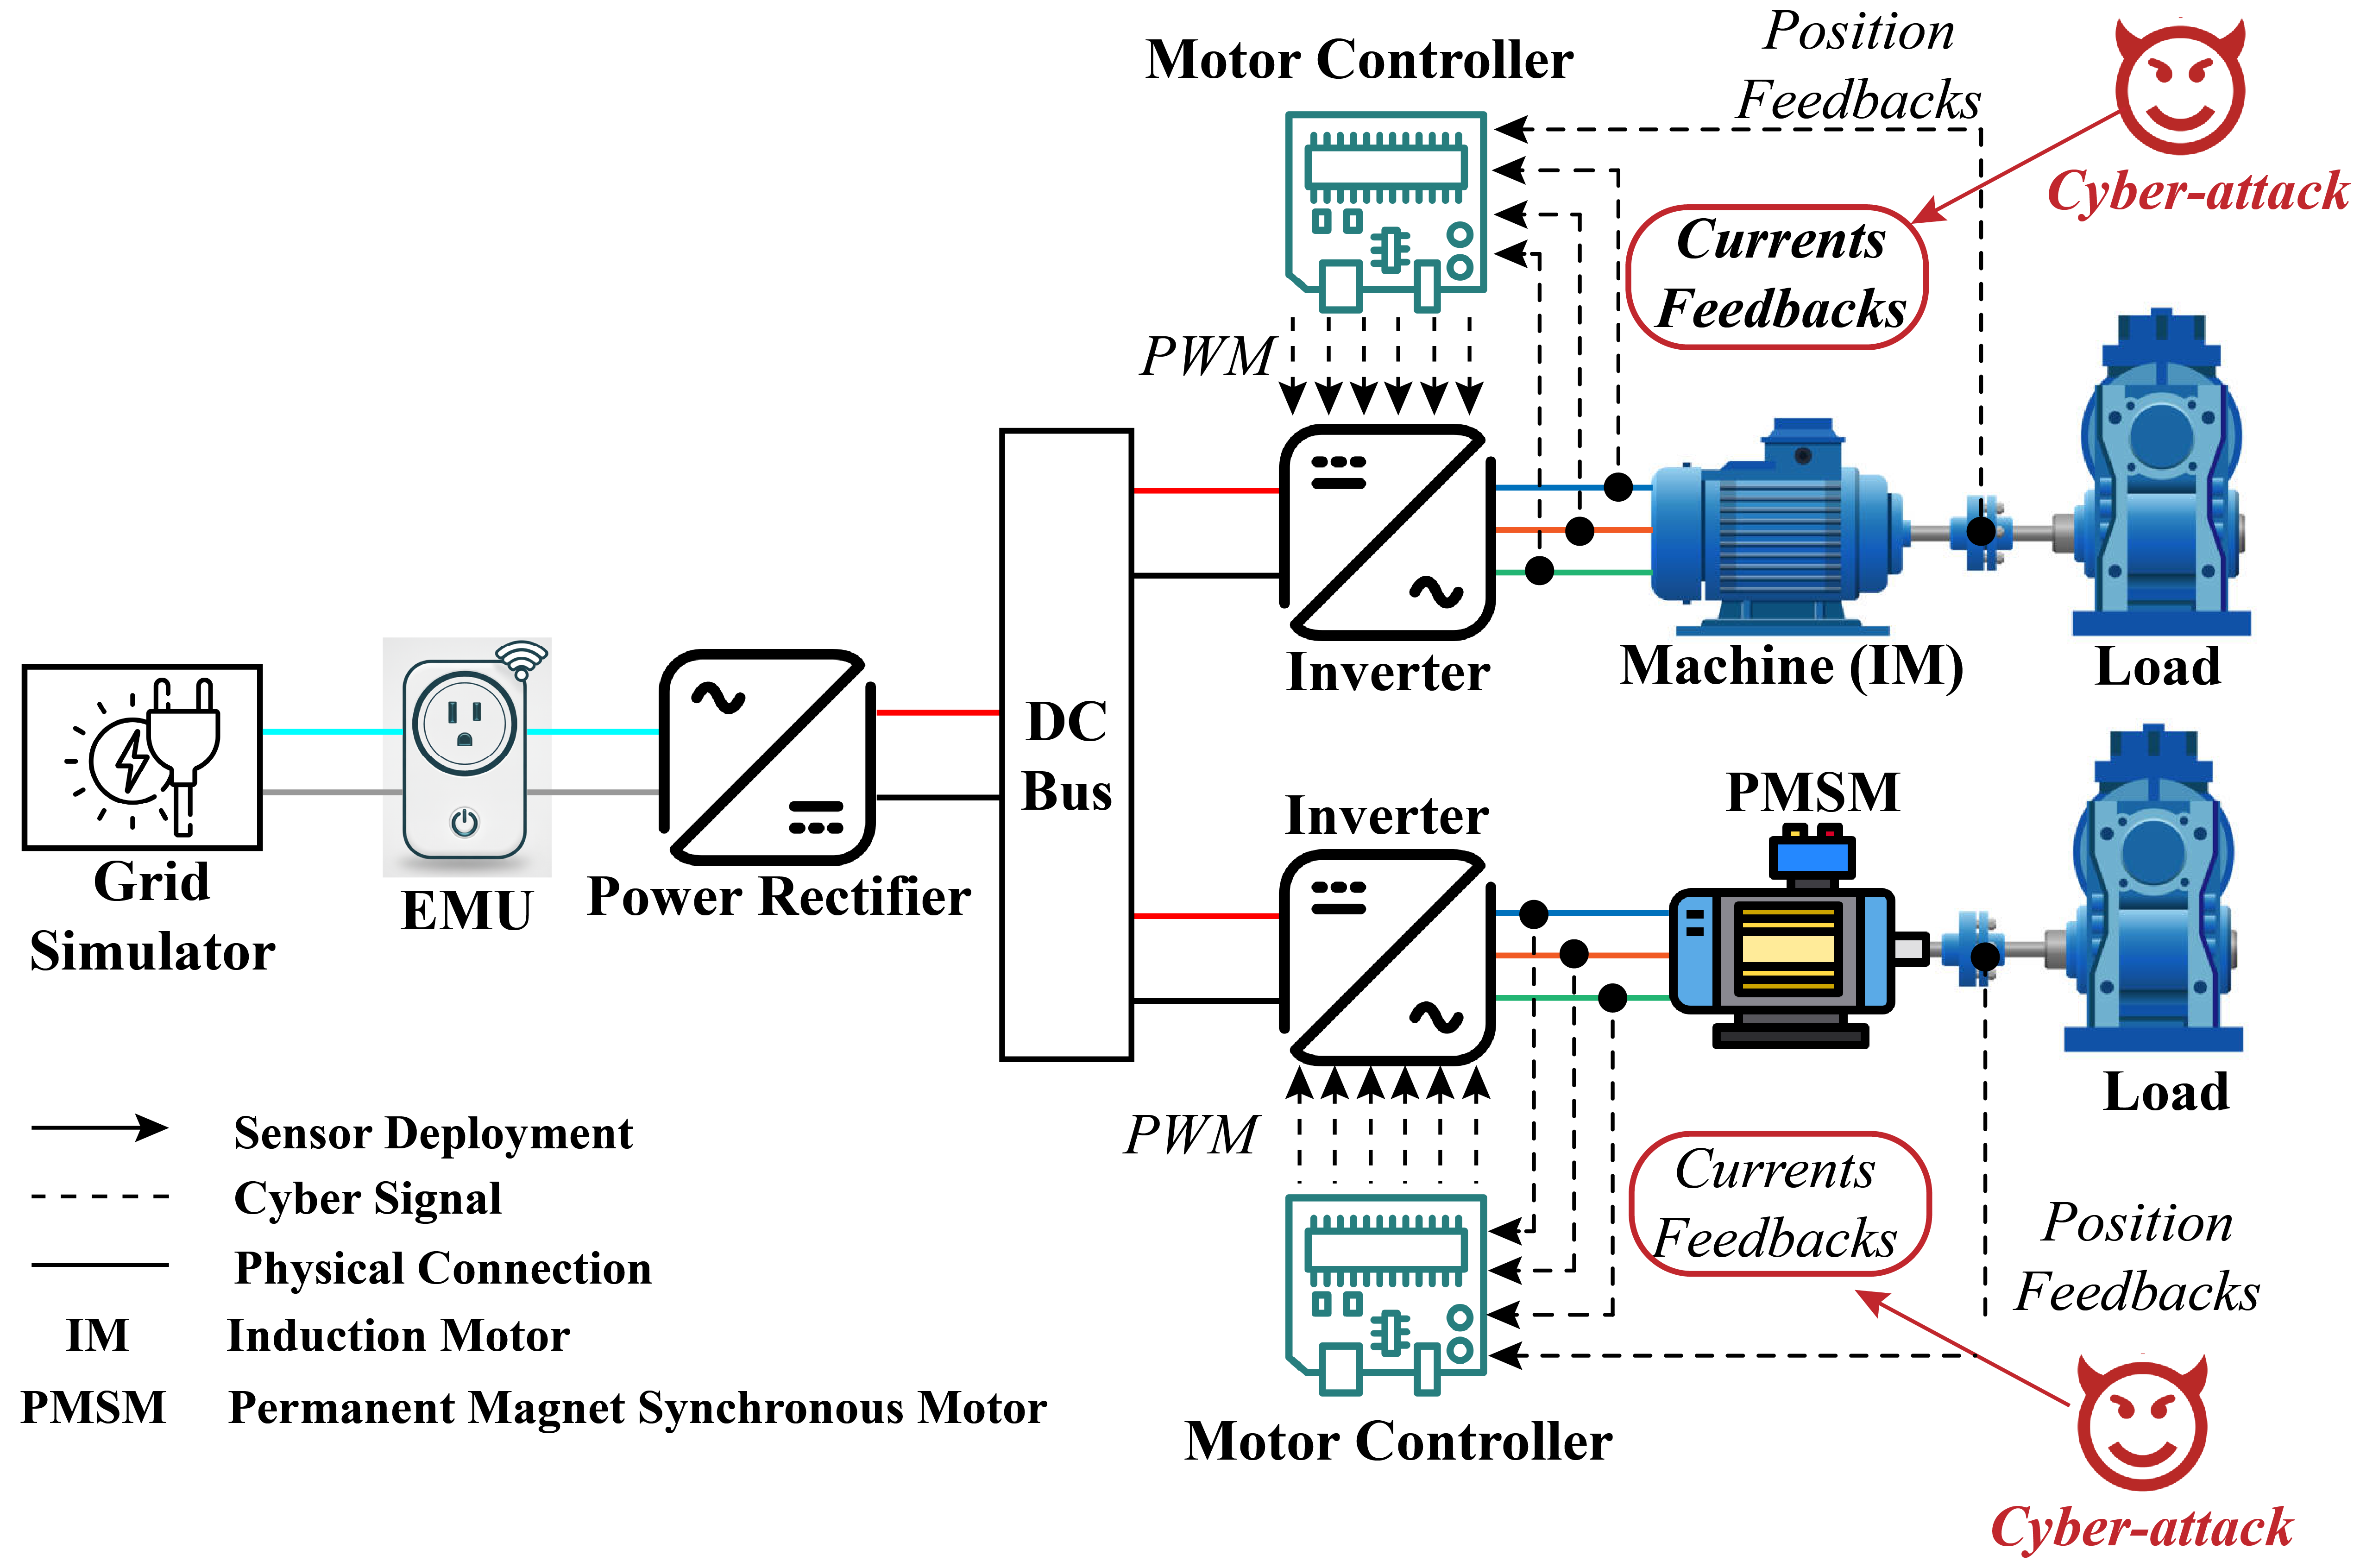
\includegraphics[width=.9\linewidth,height=.4\textheight,keepaspectratio]{figures/schematic diagram[18].png}
%DIFDELCMD <     %%%
\DIFdelendFL \DIFaddbeginFL 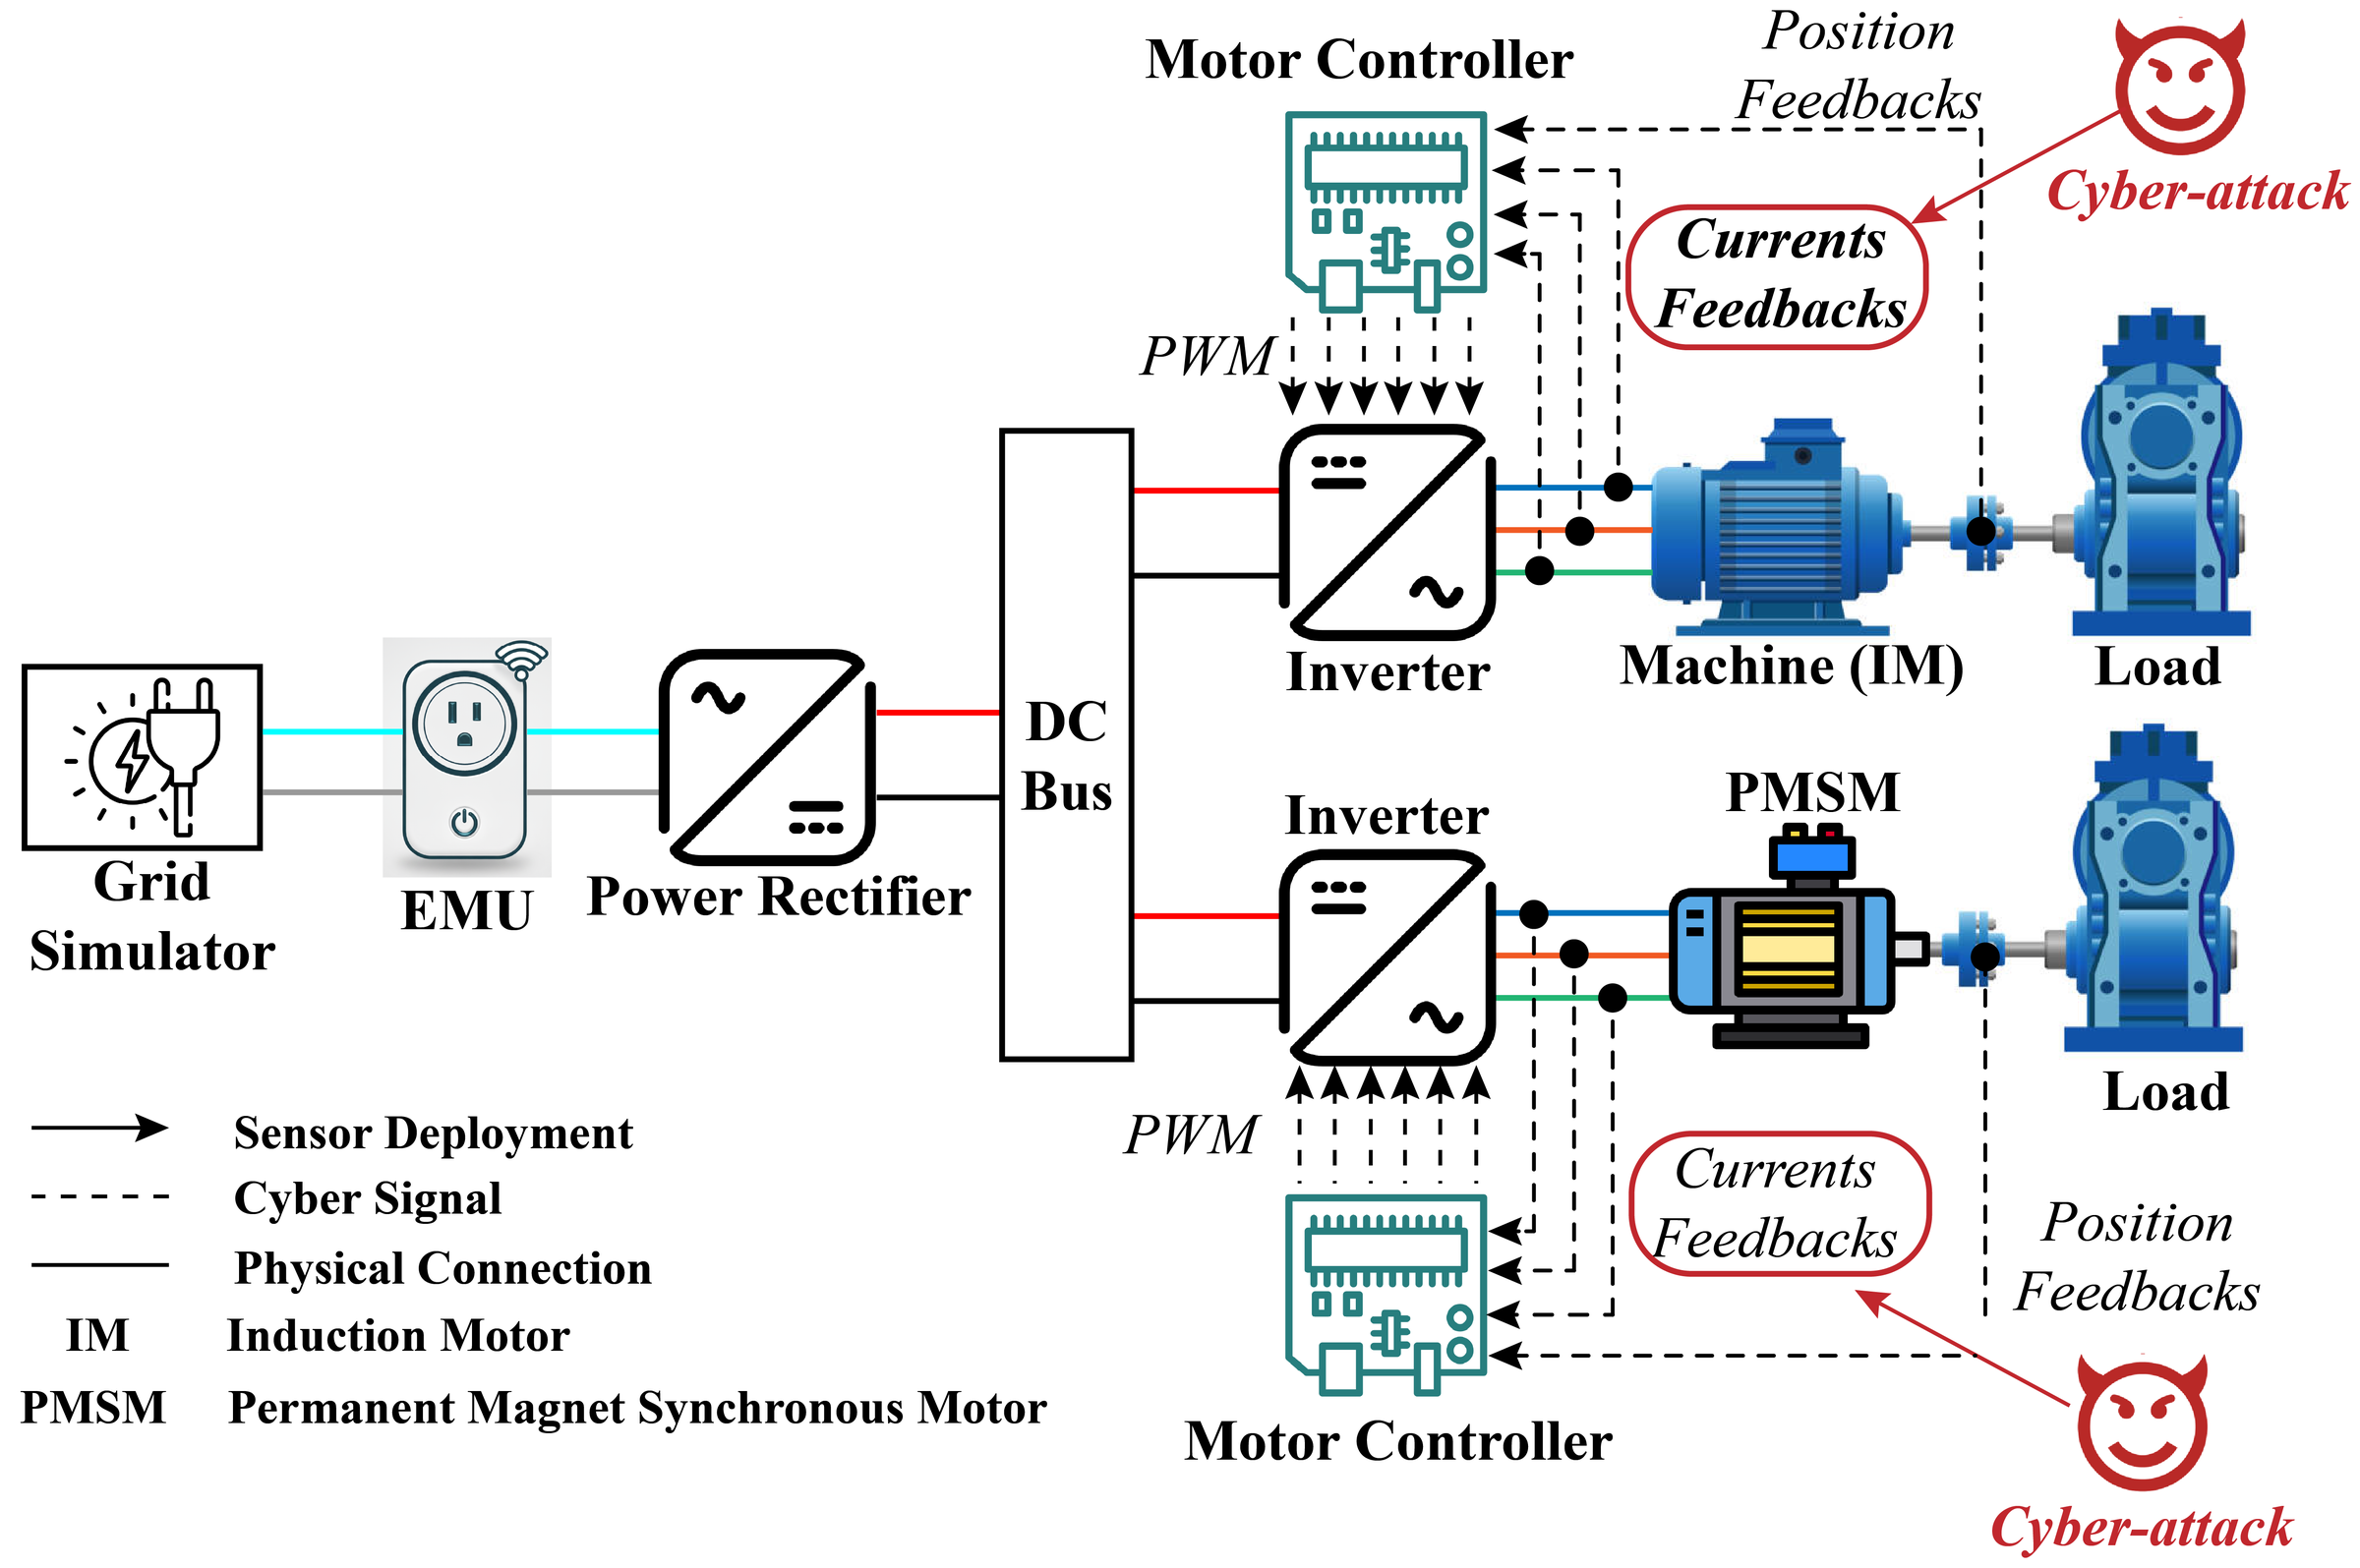
\includegraphics[width=.9\linewidth,height=.4\textheight,keepaspectratio]{figures/power_flow_apec2027.png}
    \DIFaddendFL \caption{\DIFdelbeginFL \DIFdelFL{Power Flow }\DIFdelendFL Schematic \DIFaddbeginFL \DIFaddFL{diagram of designed multi-motor testbed for applying FDIA}\DIFaddendFL }
    \label{fig:power_flow}
\end{figure}
\DIFdelbegin %DIFDELCMD < \begin{figure}[htpb]
%DIFDELCMD <     %%%
\DIFdelendFL \DIFaddbeginFL \begin{figure}[!t]
    \DIFaddendFL \centering
    \DIFdelbeginFL %DIFDELCMD < 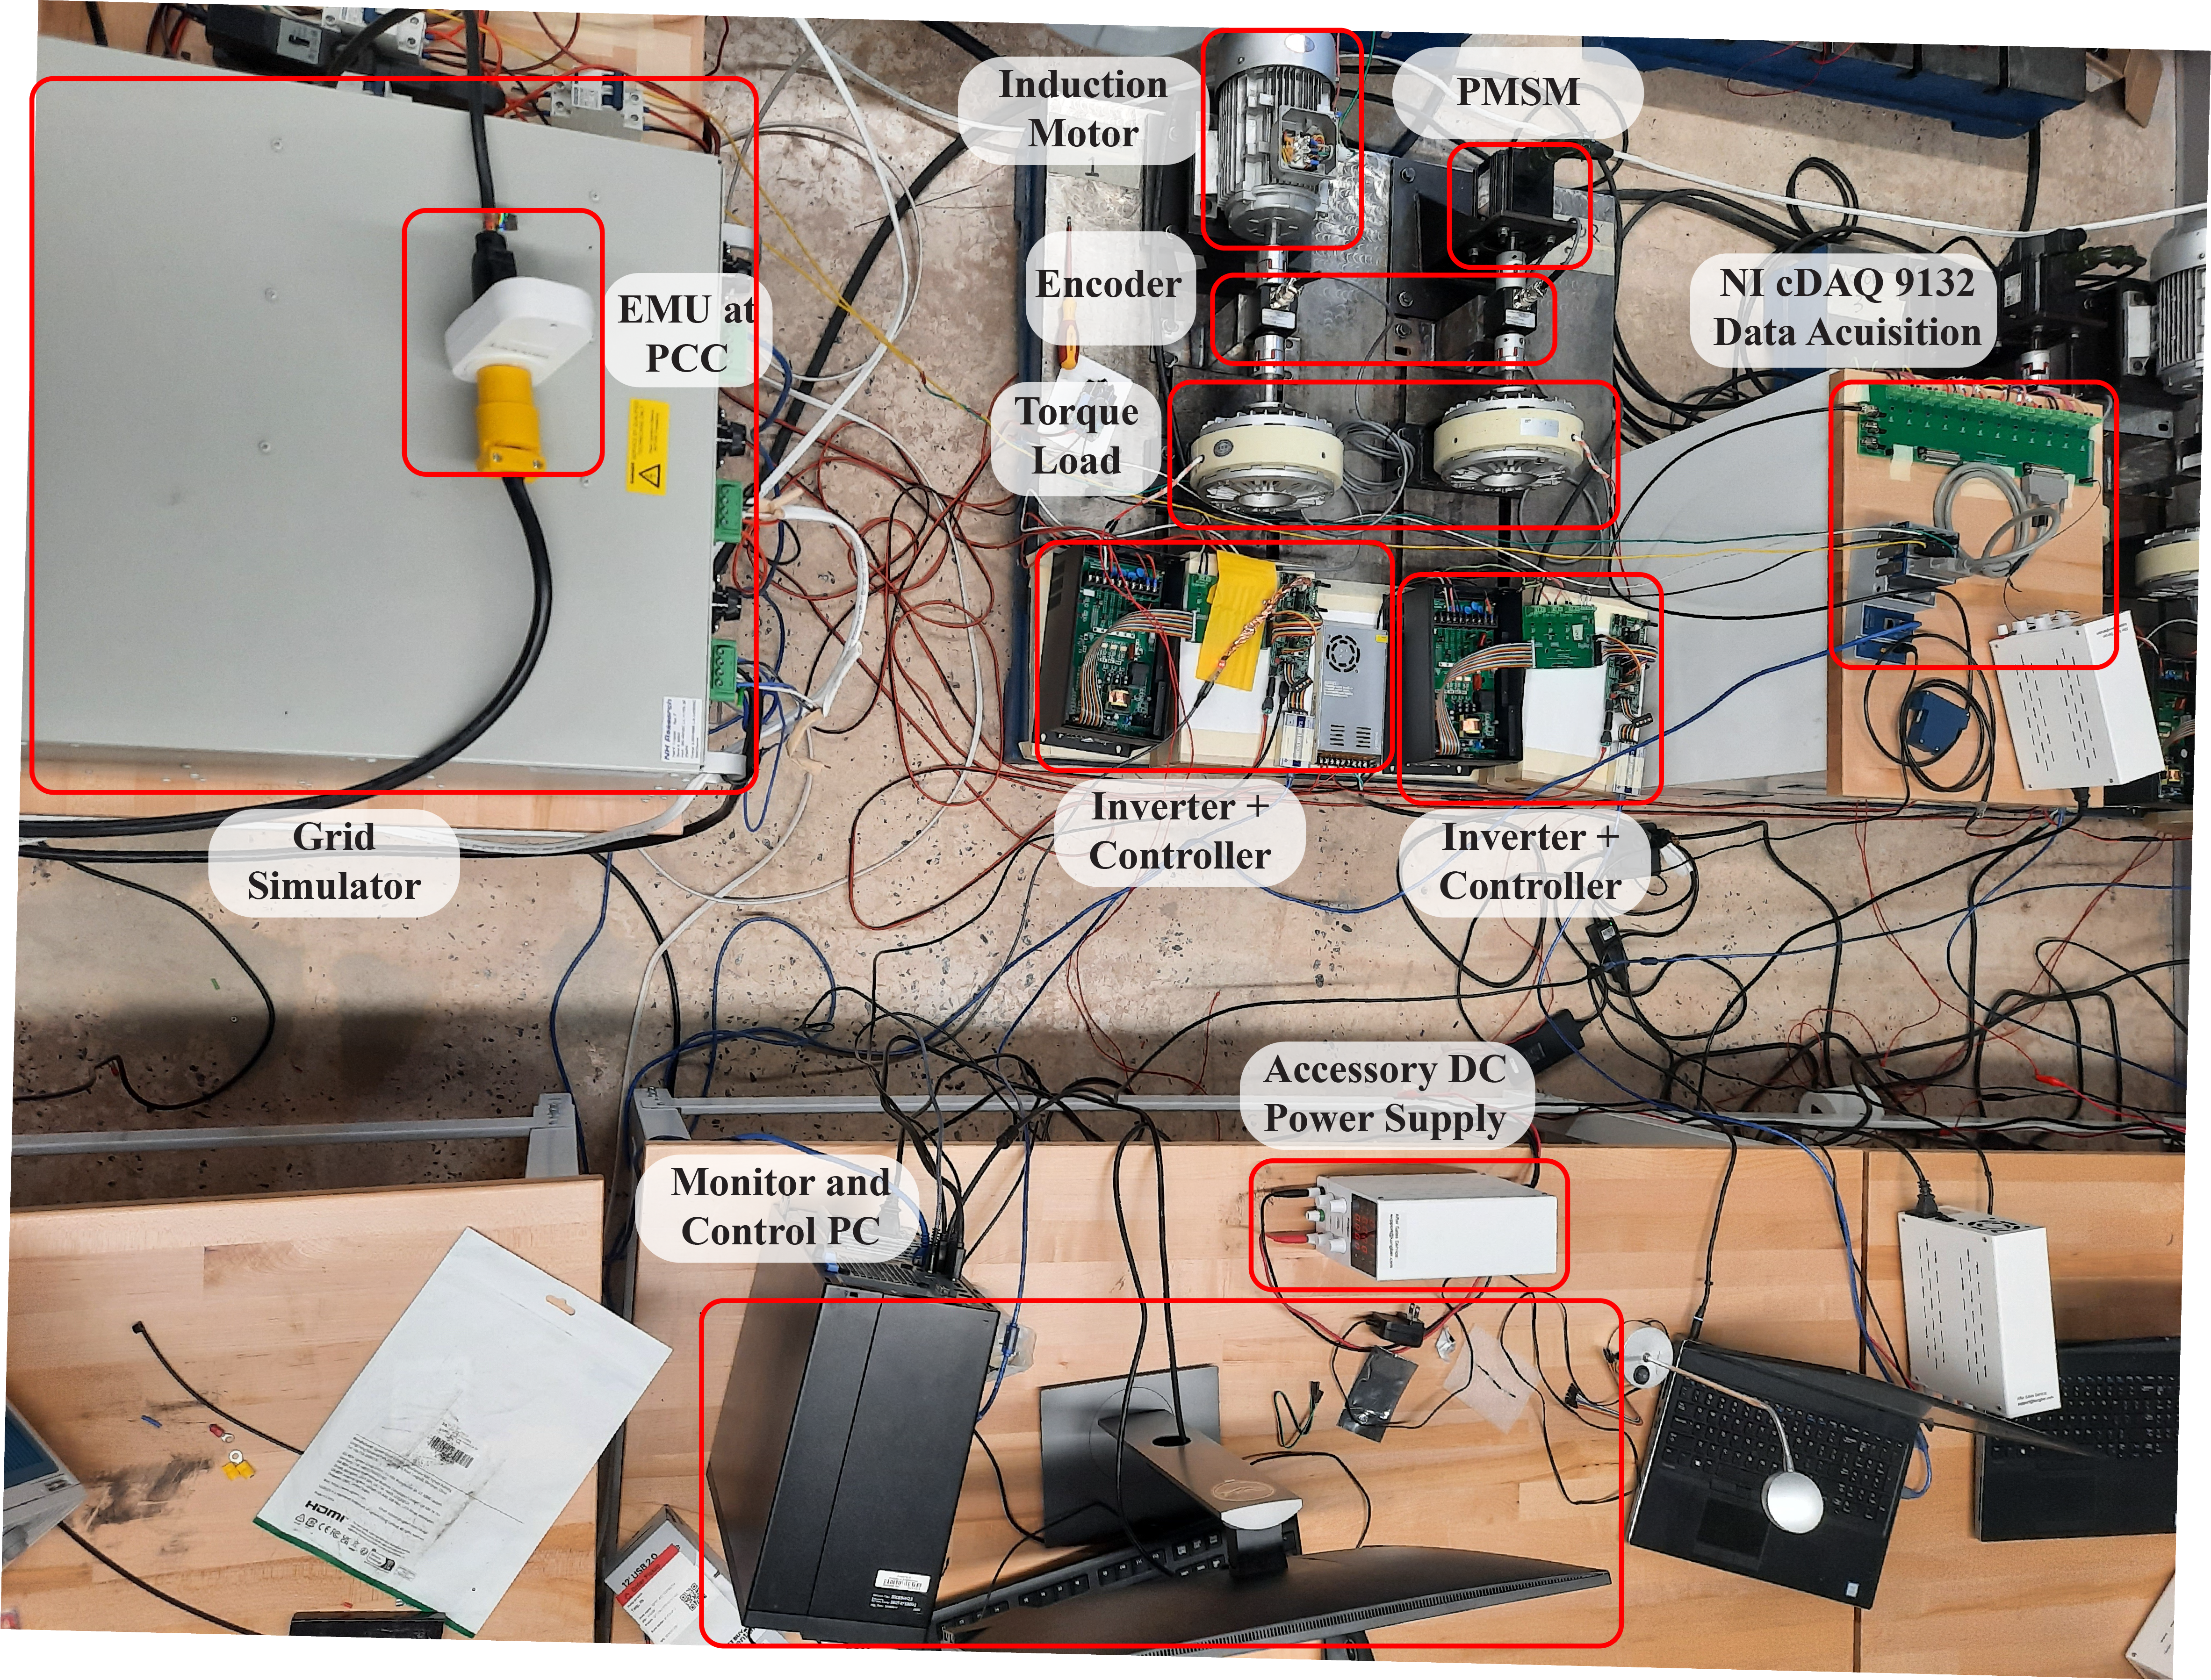
\includegraphics[width=.9\linewidth,height=.4\textheight,keepaspectratio]{figures/testbed[24].png}
%DIFDELCMD <     %%%
\DIFdelendFL \DIFaddbeginFL 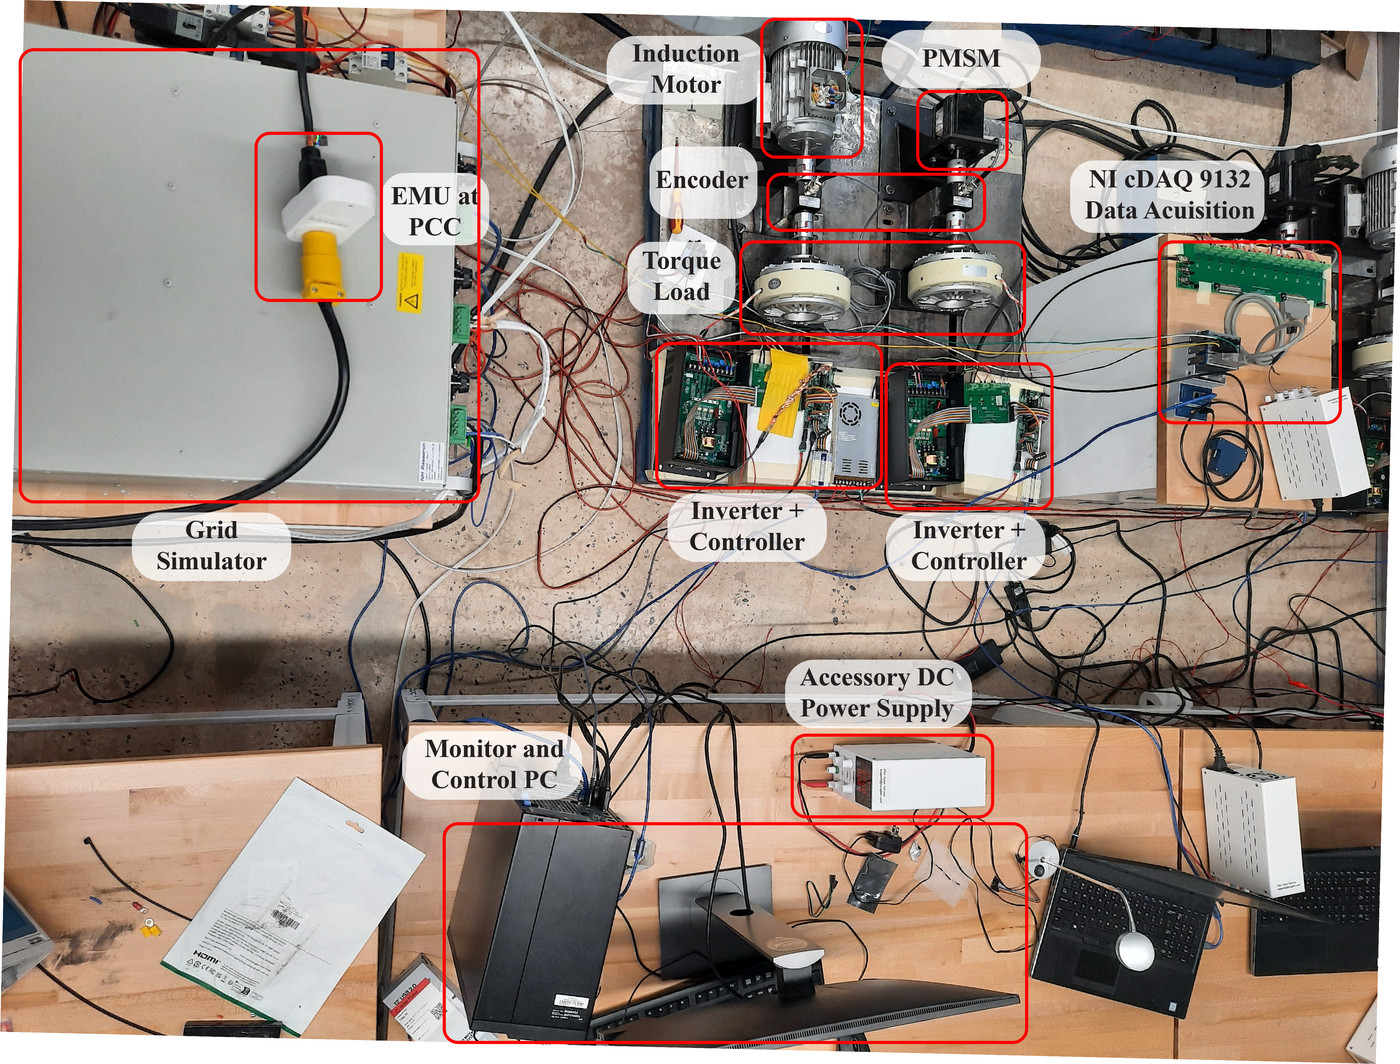
\includegraphics[width=.9\linewidth,height=.4\textheight,keepaspectratio]{figures/testbed_apec2027.jpg}
    \DIFaddendFL \caption{Physical Implementation of \DIFdelbeginFL \DIFdelFL{Power Flow}\DIFdelendFL \DIFaddbeginFL \DIFaddFL{Schematic diagram of designed multi-motor testbed}\DIFaddendFL }
    \DIFaddbeginFL \label{fig:testbed_photo}
\DIFaddendFL \end{figure}
To safely emulate cyber incidents, false data injection attacks (FDIAs) are executed through pre-embedded firmware routines that introduce an offset-style bias injection on phase-current feedback signals. The attack model is defined as:
\begin{equation}
\tilde{\mathbf{i}}_{abc}(t) = \mathbf{i}_{abc}(t) + \boldsymbol{\alpha},
\end{equation}
where $\mathbf{i}_{abc}(t)$ is the true three-phase current vector and $\boldsymbol{\alpha}$ is the injected per-unit bias (applied per phase). Trials vary operating conditions (speed and load) and injection configurations (single-phase, two-phase, and multi-point), with attack magnitudes swept over $\alpha \in \{0.00025,\ldots,0.00500\}$ pu. Each run includes steady-state operation, attack activation, and recovery, enabling scalable supervised labeling.

\subsection{Dataset Structure}
\DIFdelbegin \DIFdel{Add stride 16, the exact 16 features, the binary-label rule, metadata fields, and the dataset-schema table.
}\DIFdelend The continuous PCC time-series is segmented using an overlapping sliding window with length 128 time steps and stride 16. Each sample is represented as $X \in \mathbb{R}^{128 \times 16}$, where the 16 EMU features summarize voltage and current measurements (e.g., amplitude, phase, \DIFdelbegin \DIFdel{RMS, and THD).
}%DIFDELCMD <

%DIFDELCMD < %%%
\DIFdel{For binary detection, each window is assigned a label $y \in \{0,1\}$ derived from an \texttt{is\_attack} indicator. In addition, the dataset includes structured metadata for richer analyses, including attack onset index within the window, motor type (ACIM/PMSM), phase targeting, severity level(s}\DIFdelend \DIFaddbegin \DIFadd{root mean square (RMS}\DIFaddend ), and \DIFdelbegin \DIFdel{operating-point context (speed/load).
}\DIFdelend \DIFaddbegin \DIFadd{total harmonic distortion (THD)).
}

\DIFaddend This structure supports \DIFdelbegin \DIFdel{both }\DIFdelend real-time binary detection and \DIFdelbegin \DIFdel{future multi-class or }\DIFdelend condition-aware studies \DIFdelbegin \DIFdel{.
}%DIFDELCMD <

%DIFDELCMD < %%%
\DIFdel{Table.~\mbox{\ref{tab:dataset_schema}}summarizes the input feature groups used to construct X and the associated output labels and contextual metadata used in the dataset.
The learning task is to estimate $\hat{y}=f_{\theta}(X)$ from these labeled windows, providing a benchmark for detecting stealthy cyber-physical anomalies. }%DIFDELCMD <

%DIFDELCMD < \begin{figure}[htpb]
%DIFDELCMD <     \centering
%DIFDELCMD <     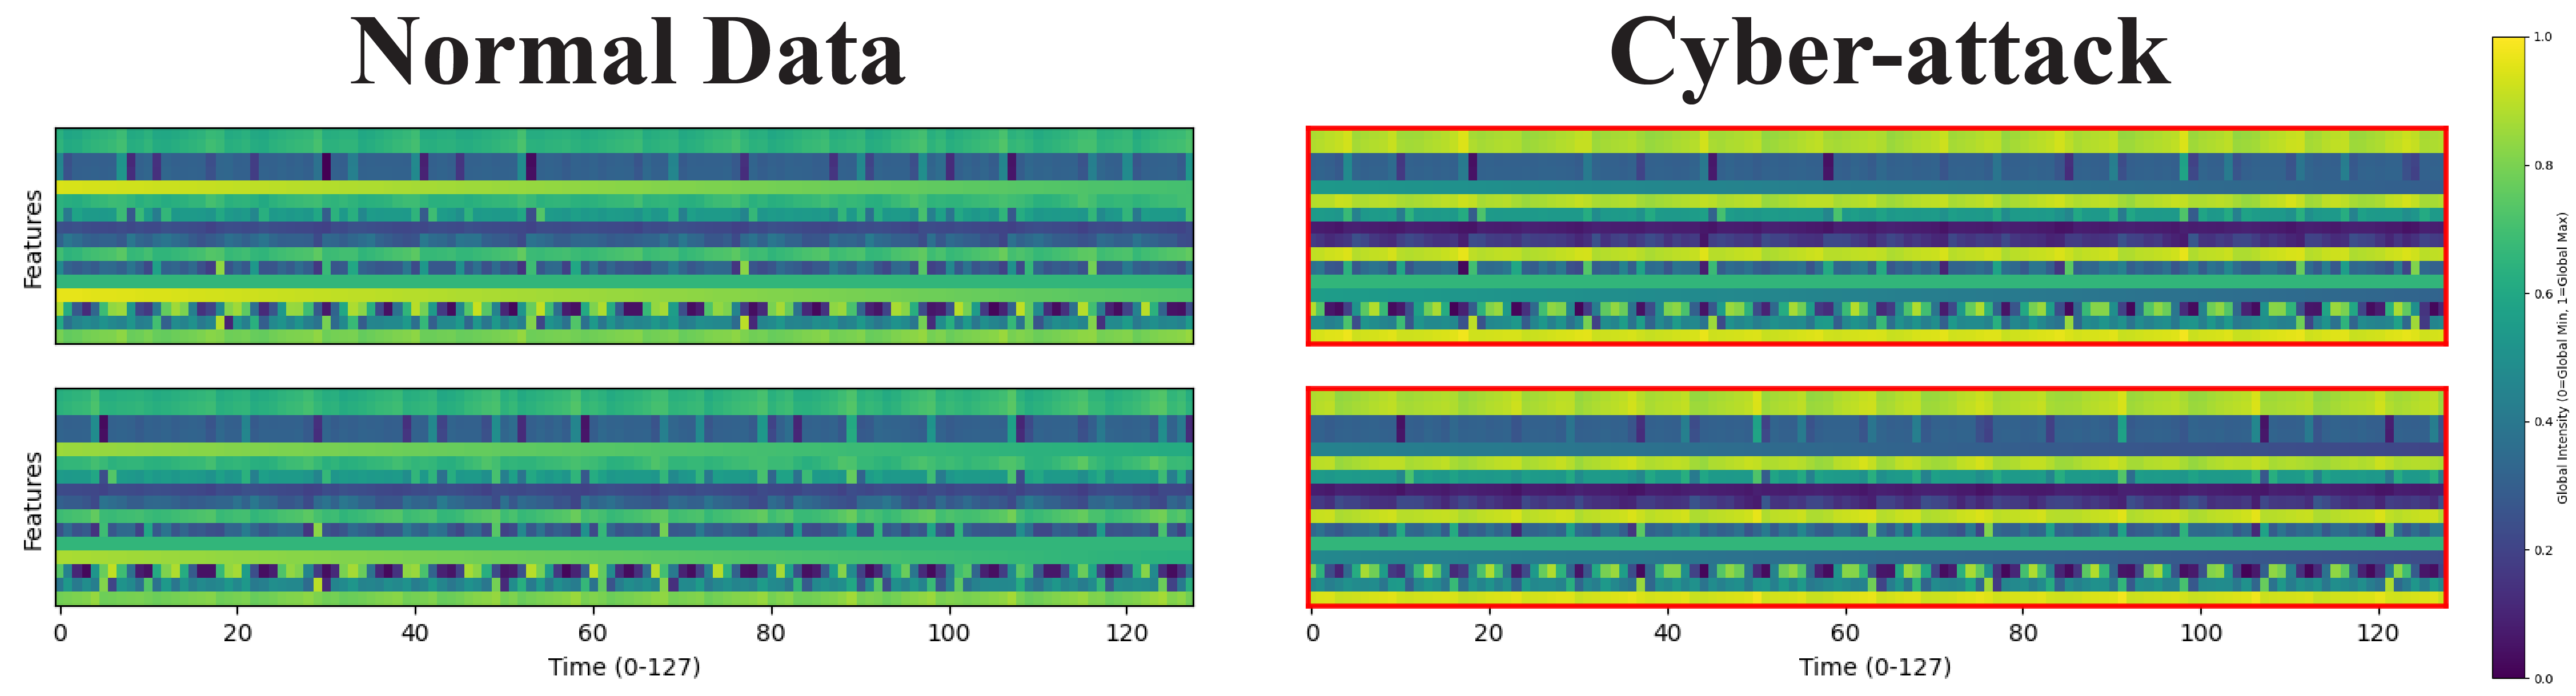
\includegraphics[width=.9\linewidth,height=.4\textheight,keepaspectratio]{figures/signals.png}
%DIFDELCMD <     %%%
%DIFDELCMD < \caption{%
{%DIFAUXCMD
\DIFdelFL{Normal vs Cyber-attack data}}
%DIFAUXCMD
%DIFDELCMD < \end{figure}
%DIFDELCMD < %%%
\DIFdel{The label vector \texttt{y} provides extensive metadata to support both binary and multi-class research objectives. Its }\DIFdelend \DIFaddbegin \DIFadd{such as motor, phase, severity and onset tasks. The }\DIFaddend 13 \DIFdelbegin \DIFdel{columns include flags for \texttt{is\_attack} (set to }\DIFdelend \DIFaddbegin \DIFadd{metadata fields are summarized in Table~\mbox{\ref{tab:dataset_schema}}. The binary label is }\DIFaddend 1 if any sample in the window is \DIFdelbegin \DIFdel{an attack), \texttt{is\_onset} (the index of }\DIFdelend \DIFaddbegin \DIFadd{attacked. Attack and phase flags are max-pooled; }\DIFaddend the first attack \DIFdelbegin \DIFdel{sample in the window), \texttt{attack\_id}, \texttt{attack\_type}, and the targeted \texttt{Motor} (encoded as 1 for ACIM, 2 for PMSM, and 0 for None).Additional columns detail the specific phasetargeted (A, B, C), the corresponding severity levels, and any speed or load alterations.This comprehensive labeling logic relies on max-pooling the metadata over the duration of the window.
}\DIFdelend \DIFaddbegin \DIFadd{index is stored as the onset label. Normal phase labels are $(A,B,C)=(0,0,0)$, and ROCOF denotes rate of change of frequency. Stored severity labels are evaluated separately from the physical injection parameter $\alpha$.
}\DIFaddend

\DIFdelbegin %DIFDELCMD < \begin{table}[H]
%DIFDELCMD < %%%
\DIFdelendFL \DIFaddbeginFL \DIFaddFL{Normal and attack feature windows are compared in Fig.~\mbox{\ref{fig:signal_windows}}; phase, frequency, and THD time-series examples are provided in Fig.~\mbox{\ref{fig:feature_timeseries}}.
}\begin{figure}[!t]
    \centering
    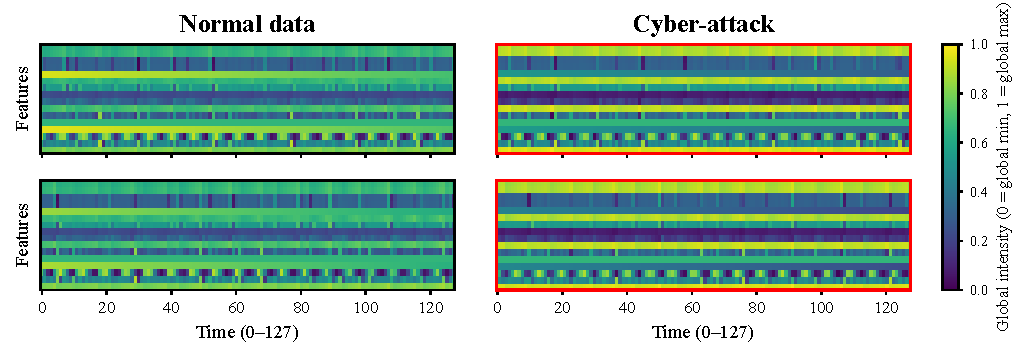
\includegraphics[width=.9\linewidth,height=.4\textheight,keepaspectratio]{figures/signals_apec2027.pdf}
    \caption{\DIFaddFL{Normal vs Cyber-attack data}}
    \label{fig:signal_windows}
\end{figure}
\begin{table*}[!t]
\DIFaddendFL \centering
\caption{Dataset Input ($X$) and Label ($y$) Schema}
\label{tab:dataset_schema}
\begin{tabular}{l|l|c}
\hline
\textbf{Input (X)} & \textbf{Features} & \textbf{Count} \\ \hline
Current Features & Amp, Amp$_2^*$, Freq, Freq$_2^*$, Phase, RMS, ROCOF, THD & 8 \\
Voltage Features & Amp, Amp$_2$, Freq, Freq$_2$, Phase, RMS, ROCOF, THD & 8 \\ \hline
\textbf{Output (y)} & \textbf{Description} & \textbf{Scope} \\
\hline
\texttt{is\_attack} & Binary (0=Normal, 1=Attack) & 2 \\
\texttt{is\_onset} & First attack index \DIFdelbeginFL \DIFdelFL{in window }\DIFdelendFL (0--127)\DIFaddbeginFL \DIFaddFL{; $-1$ if absent }\DIFaddendFL & \DIFdelbeginFL \DIFdelFL{128 }\DIFdelendFL \DIFaddbeginFL \DIFaddFL{$128+1$ }\DIFaddendFL \\
\texttt{attack\_type} & Attack mode (normal:0, cyber\_attack:1) & 2 \\
\texttt{Motor} & 0=None, 1=ACIM, 2=PMSM & 3 \\
\texttt{A, B, C} & Phase-specific injection flags (0 and 1) & 2 \\
$\text{sev}_A, \text{sev}_B, \text{sev}_C$ & \DIFdelbeginFL \DIFdelFL{Intensity }\DIFdelendFL \DIFaddbeginFL \DIFaddFL{Stored severity }\DIFaddendFL per phase (\DIFdelbeginFL \DIFdelFL{0.00025, 0.00050}\DIFdelendFL \DIFaddbeginFL \DIFaddFL{0.025, 0.050}\DIFaddendFL , \ldots, \DIFdelbeginFL \DIFdelFL{0.00500}\DIFdelendFL \DIFaddbeginFL \DIFaddFL{0.500}\DIFaddendFL ) & 20 \\
\texttt{speed} & Motor speed settings (700, 1000, and 1300 RPM) & 3 \\
\texttt{load} & Motor torque load settings (2, 3, and 4) & 3 \\
\texttt{attack\_id} & Unique event identifier & \DIFdelbeginFL \DIFdelFL{2730 }\DIFdelendFL \DIFaddbeginFL \DIFaddFL{2727 }\DIFaddendFL \\ \hline
\multicolumn{3}{l}{$^*$Amp$_2$ and Freq$_2$ denote the second dominant amplitude and frequency components.} \\
\end{tabular}
\DIFdelbeginFL %DIFDELCMD < \end{table}
%DIFDELCMD <

%DIFDELCMD < \begin{figure}[h]
%DIFDELCMD <     %%%
\DIFdelendFL \DIFaddbeginFL \end{table*}
\begin{figure}[!t]
    \DIFaddendFL \centering
    \DIFdelbeginFL %DIFDELCMD < 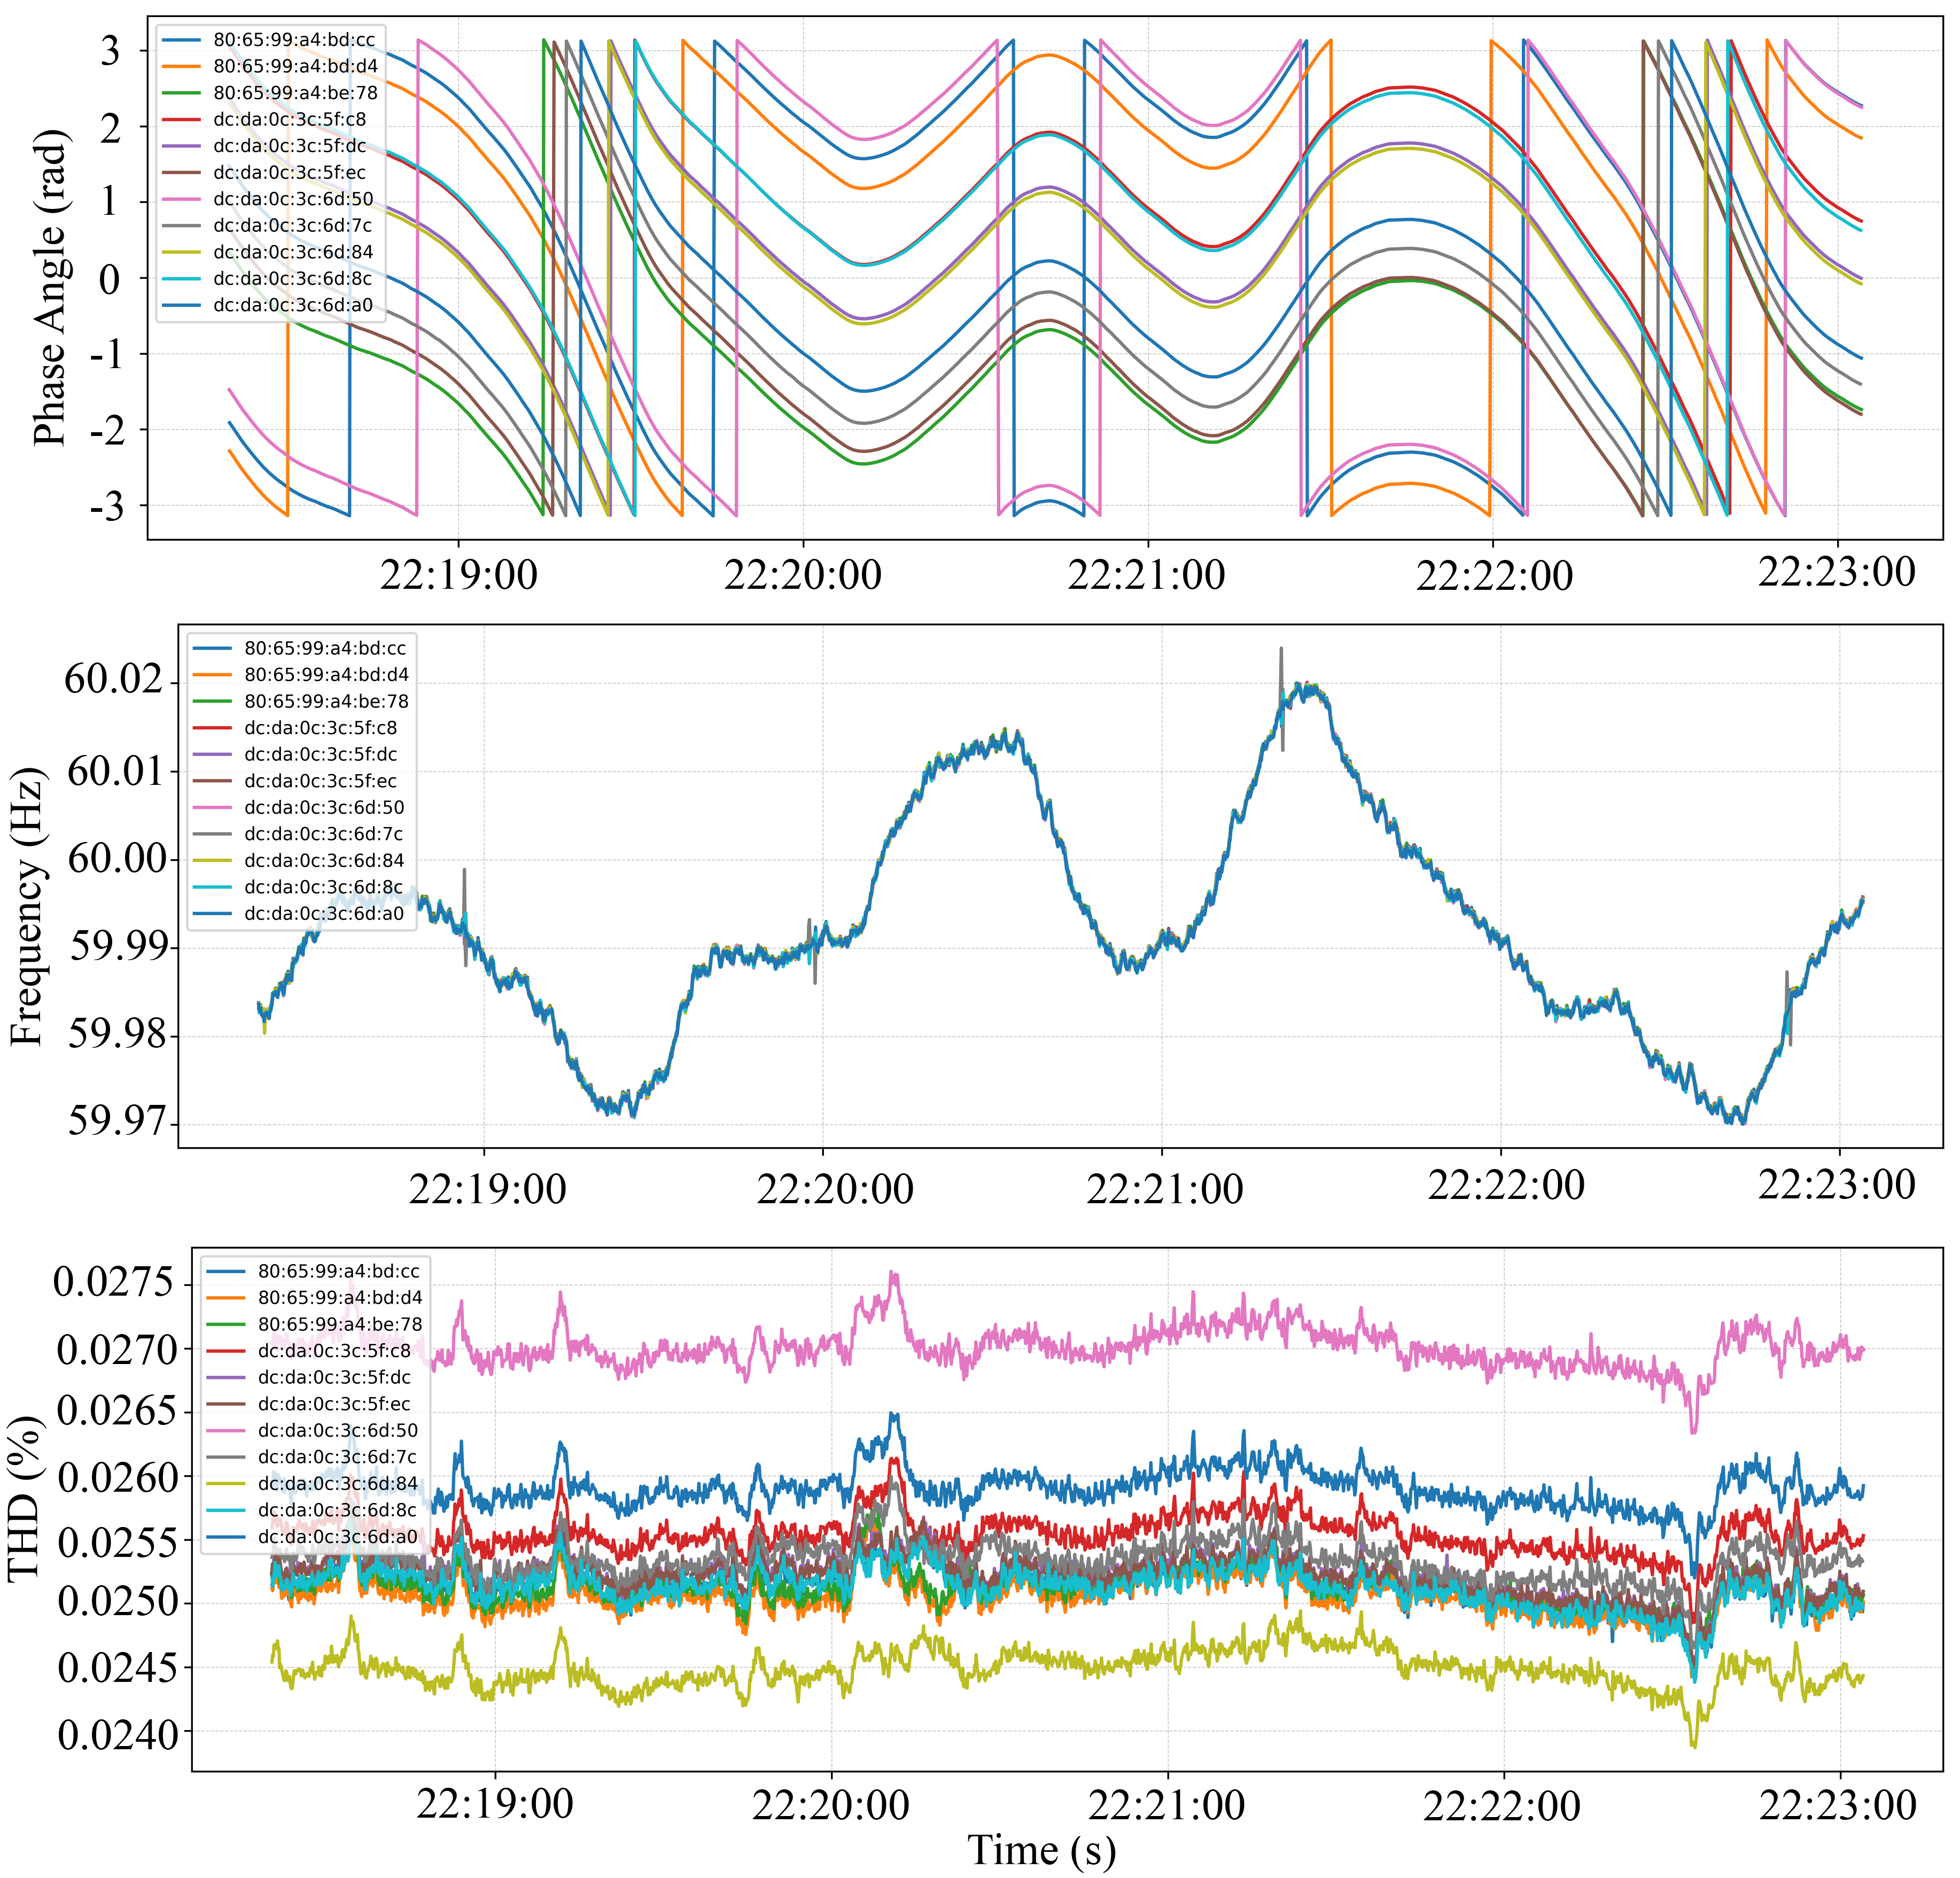
\includegraphics[width=.9\linewidth,height=.4\textheight,keepaspectratio]{featurescombined.png}
%DIFDELCMD <     %%%
\DIFdelendFL \DIFaddbeginFL 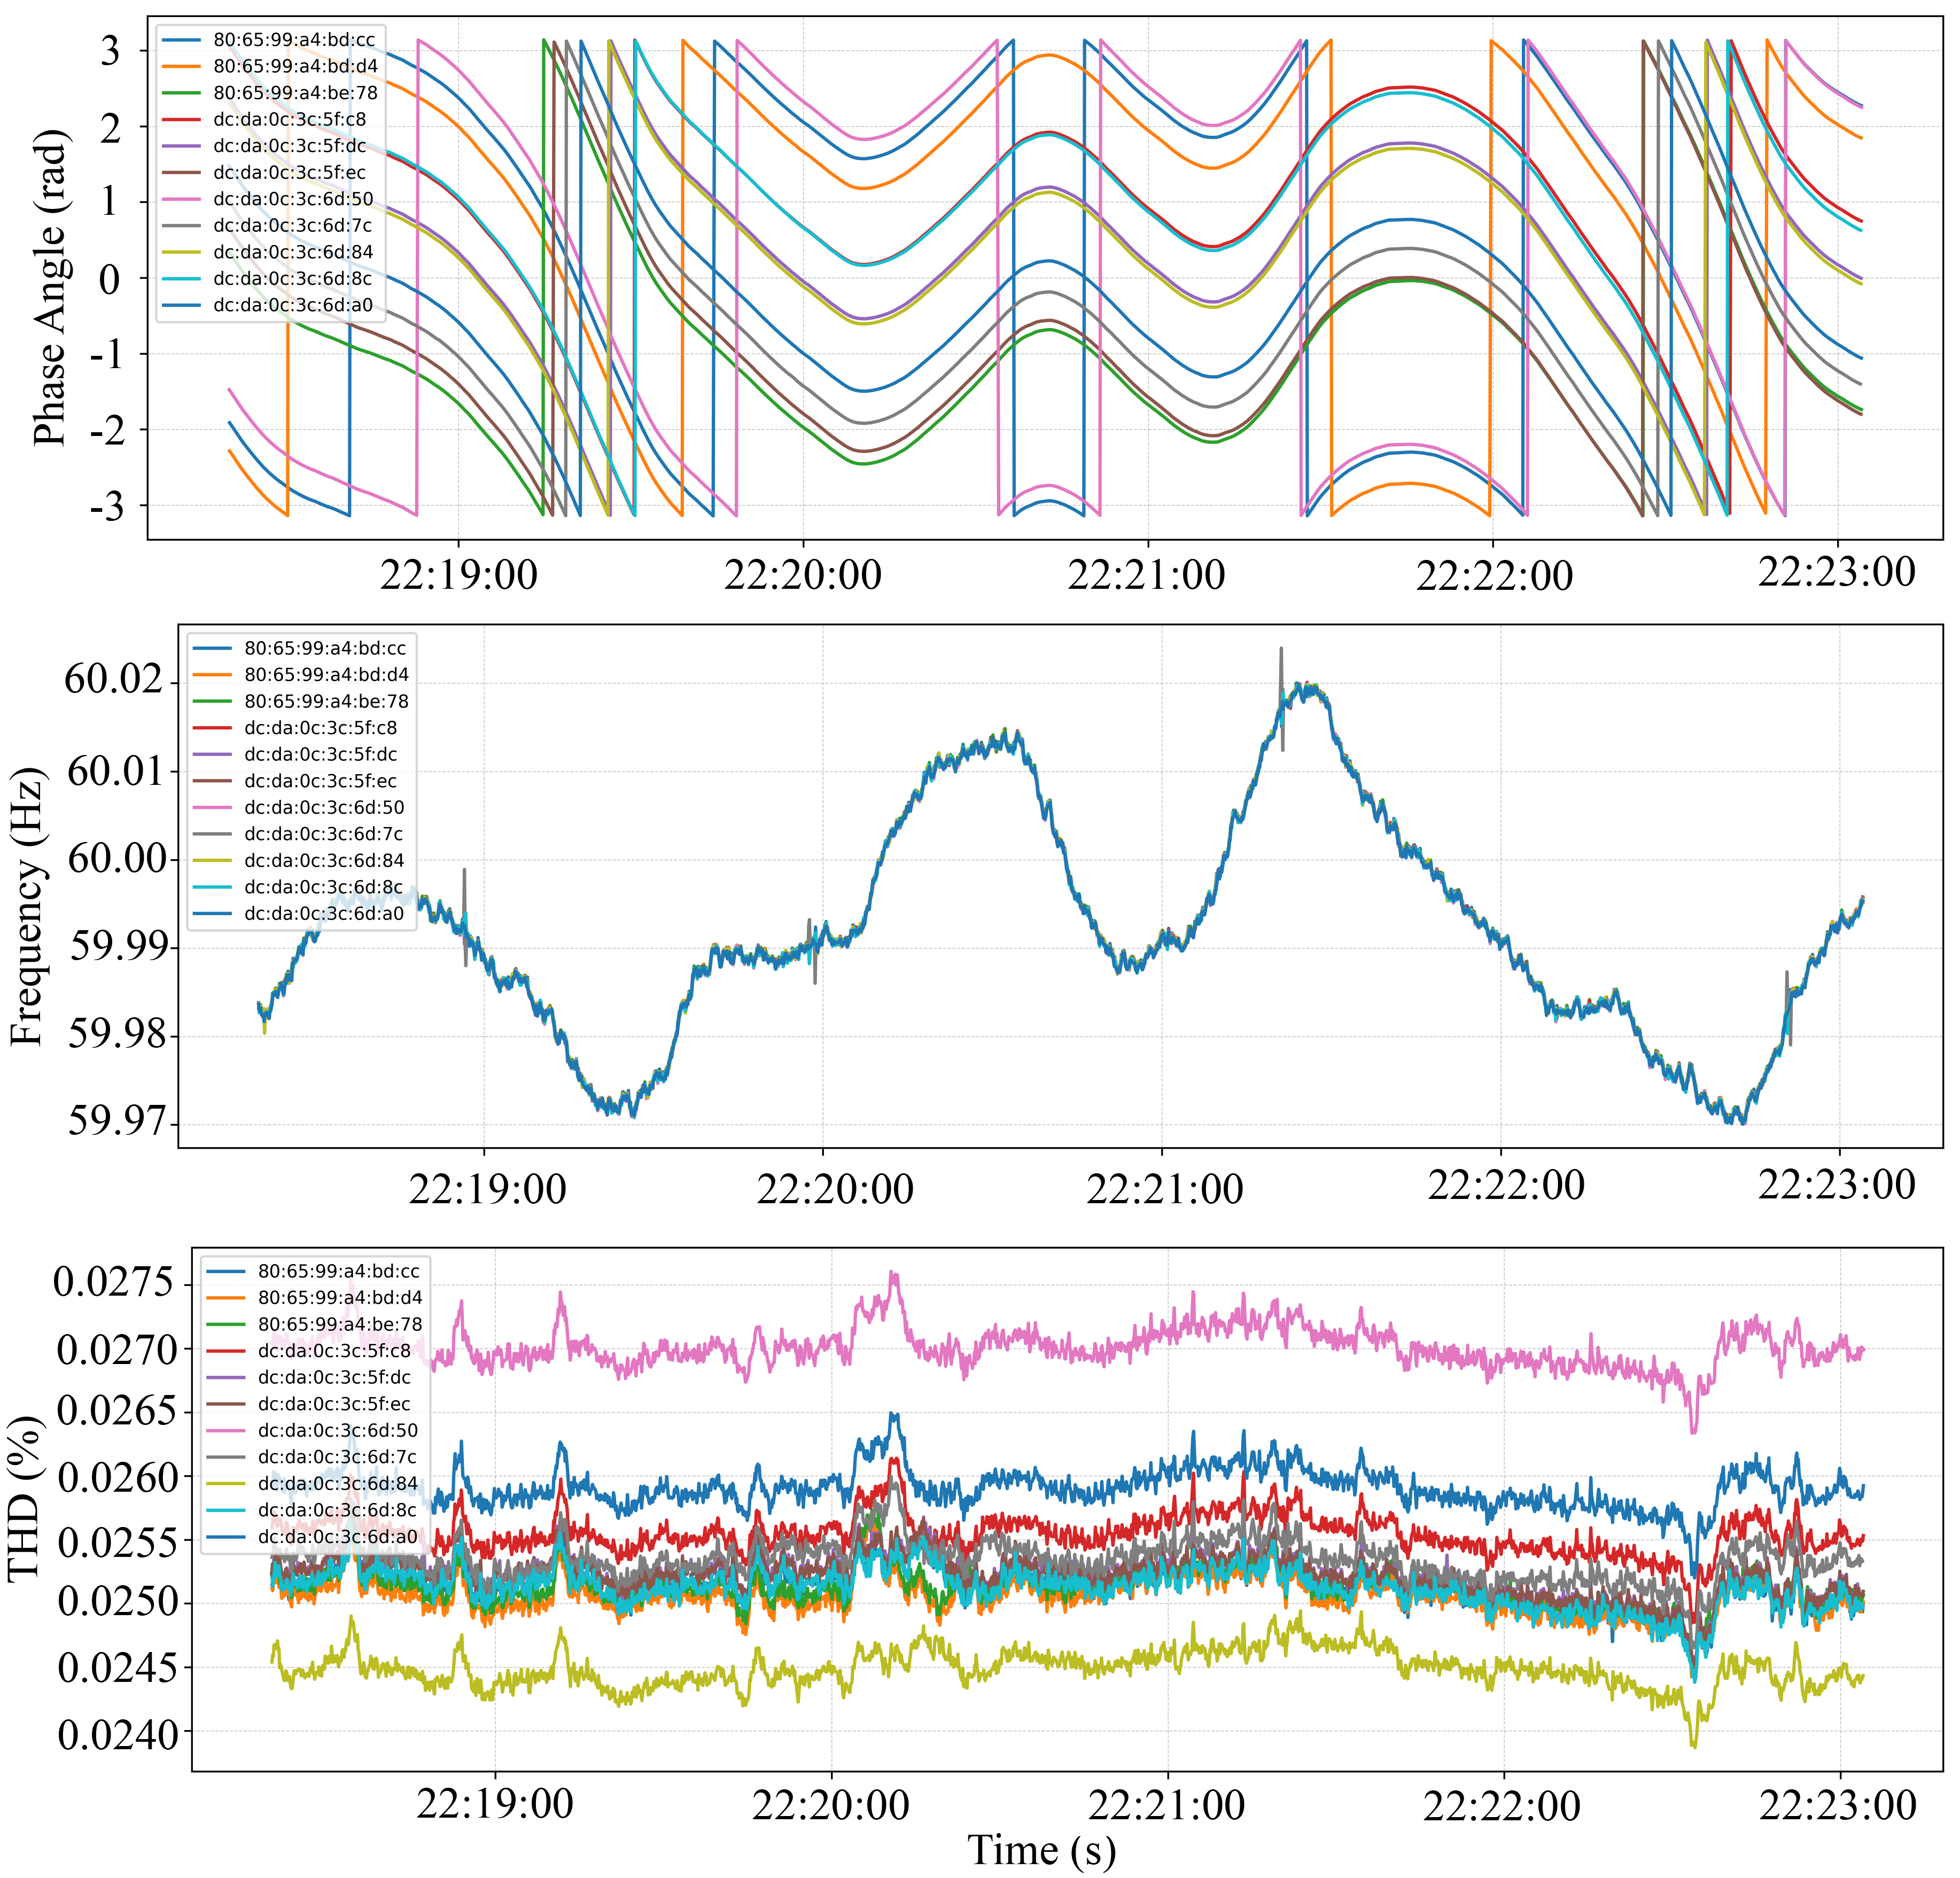
\includegraphics[width=.9\linewidth,height=.4\textheight,keepaspectratio]{featurescombined.png}
    \DIFaddendFL \caption{Comparative time-series visualization \DIFdelbeginFL \DIFdelFL{distinguishing normal operational baseline sequences from injected cyber anomalies}\DIFdelendFL \DIFaddbeginFL \DIFaddFL{of EMU phase, frequency, and THD measurements}\DIFaddendFL .}
    \DIFaddbeginFL \label{fig:feature_timeseries}
\DIFaddendFL \end{figure}

\section{Bidirectional GRU Architecture}

\DIFdelbegin \DIFdel{Recurrent models are well-suited for EMU time-series classification because cyber anomalies often manifest as }\DIFdelend \DIFaddbegin \DIFadd{A CNN--Bi-GRU network is used because }\DIFaddend subtle temporal deviations \DIFdelbegin \DIFdel{rather than }\DIFdelend \DIFaddbegin \DIFadd{must be distinguished from }\DIFaddend isolated point events. \DIFdelbegin \DIFdel{We initially evaluated an LSTM baseline, but adopted a Bidirectional GRU (Bi-GRU) to reduce gating complexity while capturing contextual dependencies across each }\DIFdelend \DIFaddbegin \DIFadd{Gated recurrence~\mbox{\cite{cho2014}} and bidirectional sequence processing~\mbox{\cite{schuster1997}} are combined within each completed }\DIFaddend observation window.

\DIFdelbegin \DIFdel{Prior to training, each EMU sample is a fixed-length sequence. We augment each window by concatenating first-order temporal differences along the feature axis (from $128\times16$ to $128\times32$), followed by feature-wise standardization using statistics from the training split. The overall data acquisition, preprocessing , and model inference pipeline is }\DIFdelend \DIFaddbegin \DIFadd{The preprocessing and shared six-head network are }\DIFaddend illustrated in Fig.~\mbox{\ref{architecture}}. \DIFaddbegin \DIFadd{Each $128\times16$ window is expanded to $128\times32$ by the temporal feature construction described below.
}\DIFaddend The classifier comprises two Conv1D blocks (64 filters, kernel size 3) with Batch Normalization, followed by a Bidirectional GRU for sequence modeling. \DIFaddbegin \DIFadd{Local temporal patterns are extracted by Conv1D filters across input channels. Retained state is controlled by GRU update/reset gates, and each completed window is processed forward and backward to combine context. }\DIFaddend Outputs are aggregated with GlobalAveragePooling1D, passed through a 64-unit dense layer with 30\% dropout, and mapped to \DIFdelbegin \DIFdel{a sigmoidnode for binary classification. }%DIFDELCMD < \begin{figure}[H]
%DIFDELCMD <     %%%
\DIFdelendFL \DIFaddbeginFL \DIFaddFL{six parallel heads: attack (one sigmoid), motor (two-class softmax), phases (three sigmoids), severity (three sigmoids), start presence (one sigmoid), and start position (one sigmoid). The shared Bi-GRU has 64 units per direction; the model has 77,963 parameters.
}\begin{figure*}[t]
    \DIFaddendFL \centering
    \DIFdelbeginFL %DIFDELCMD < 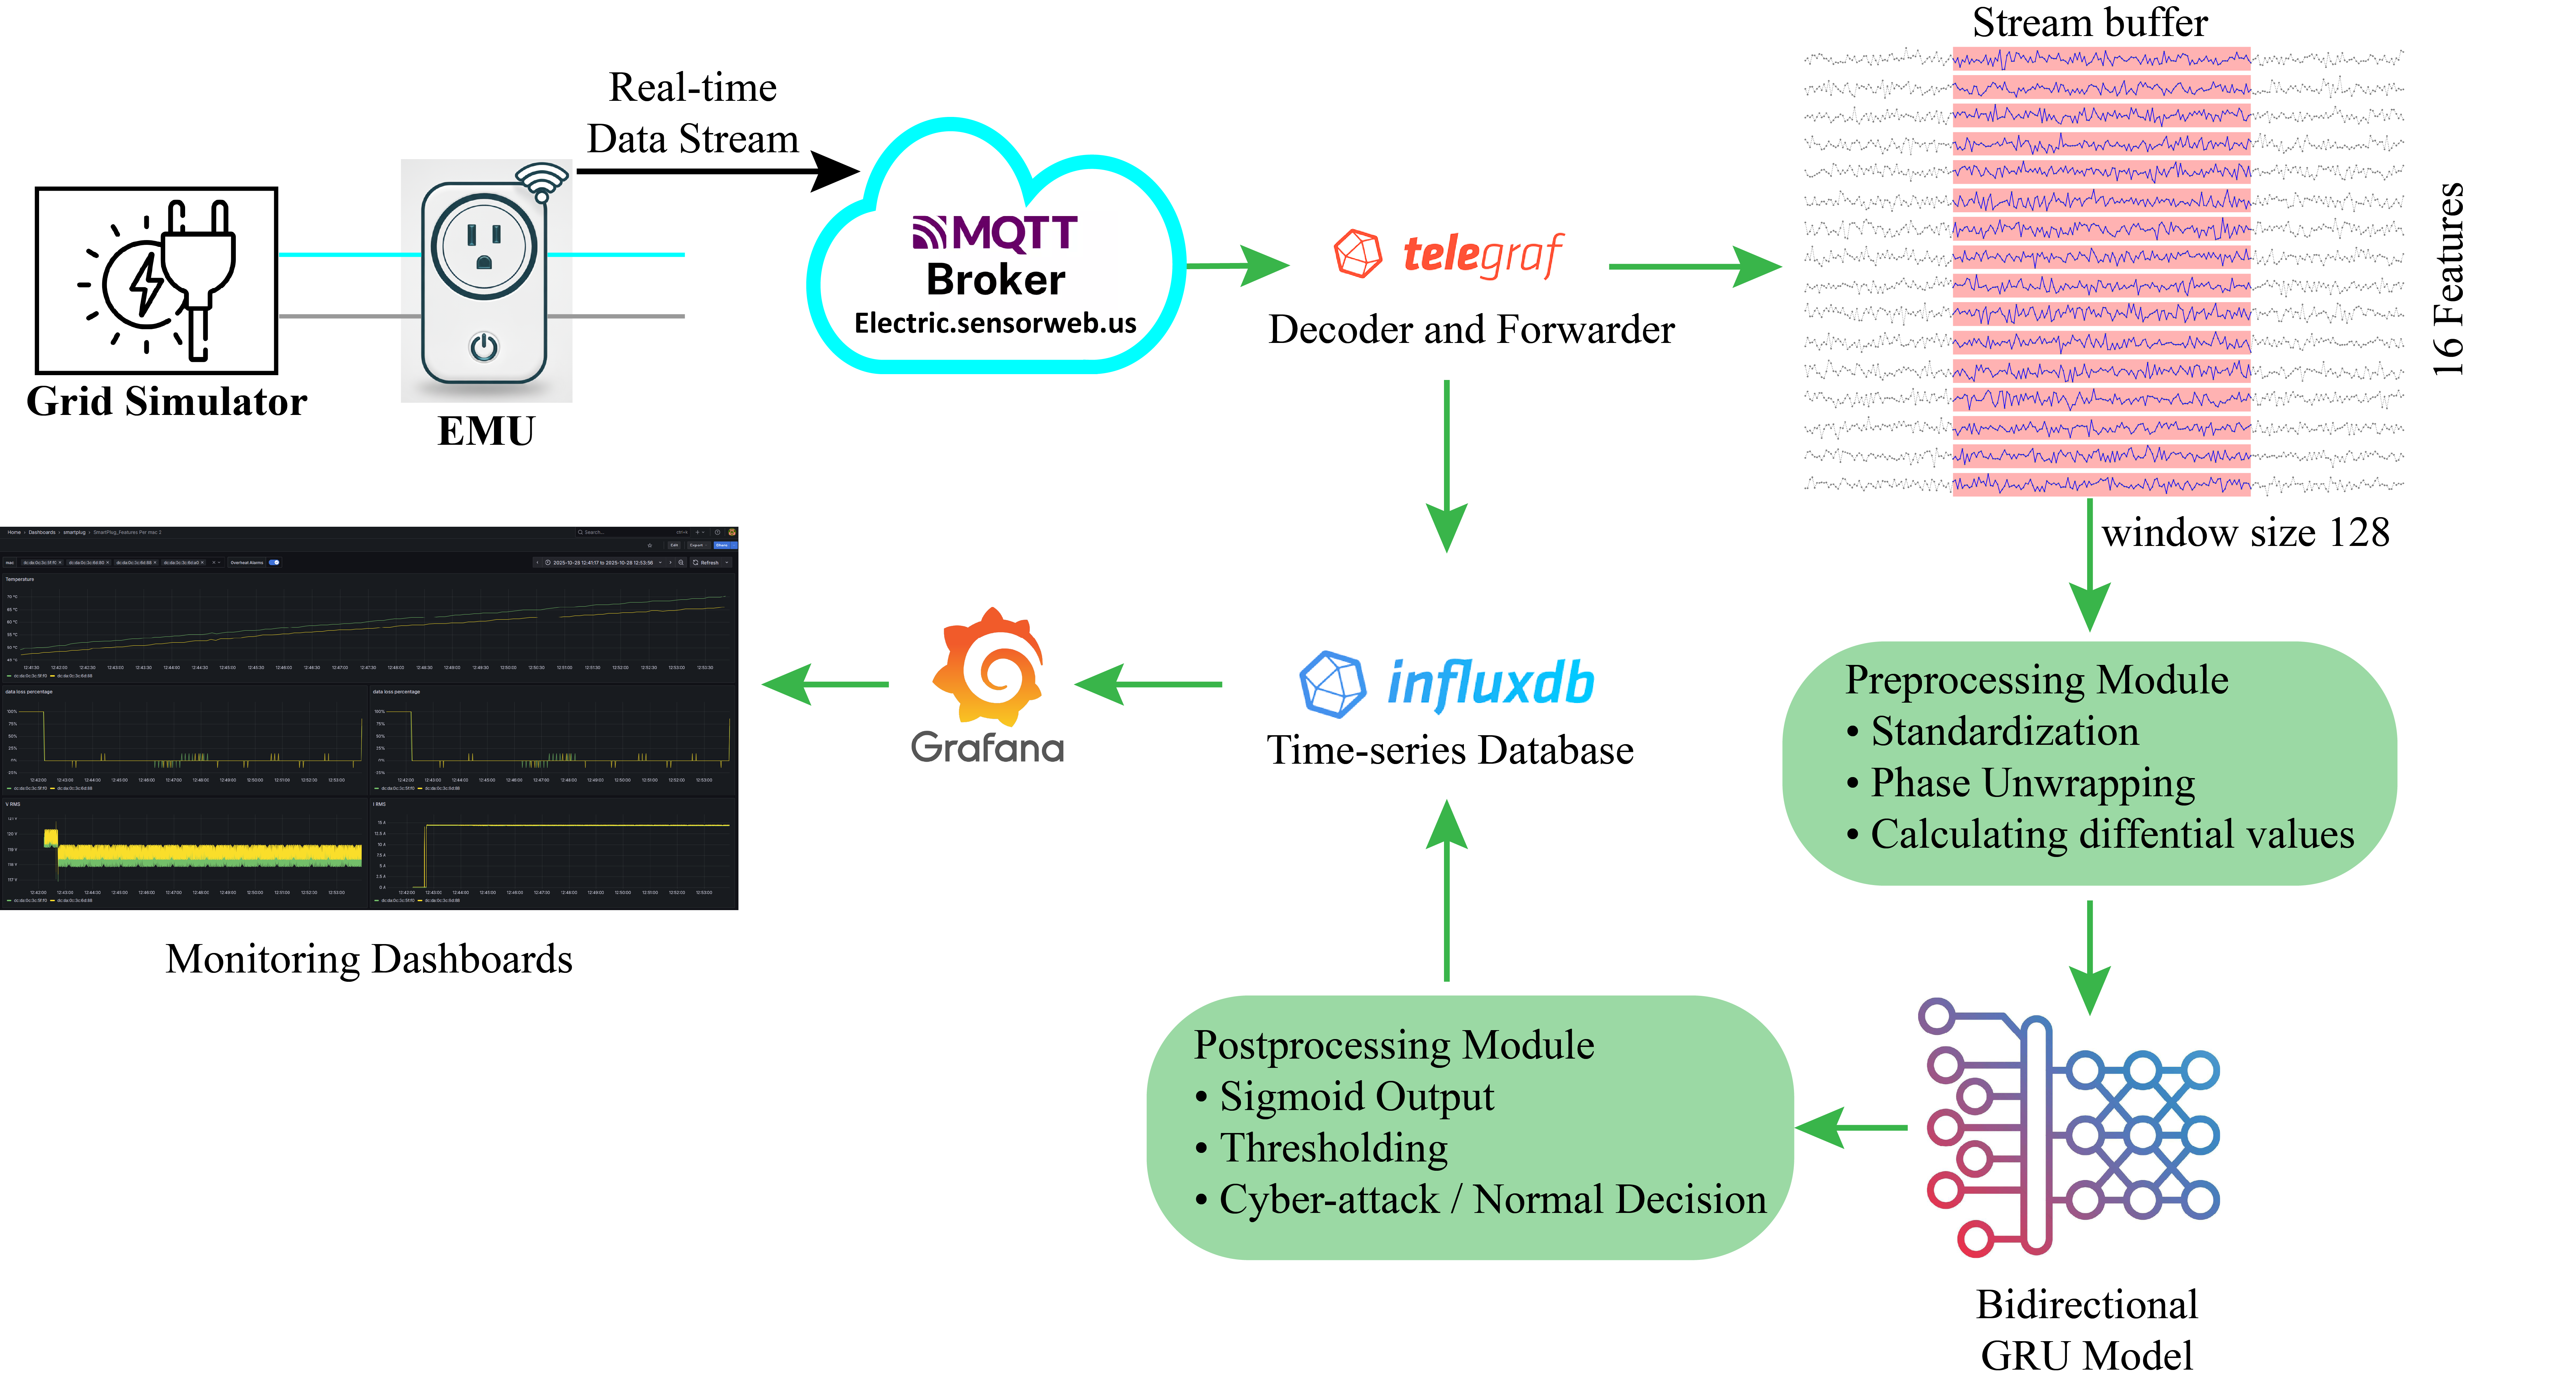
\includegraphics[width=.9\linewidth,height=.4\textheight,keepaspectratio]{figures/schematic diagram.png}
%DIFDELCMD <     %%%
\DIFdelendFL \DIFaddbeginFL 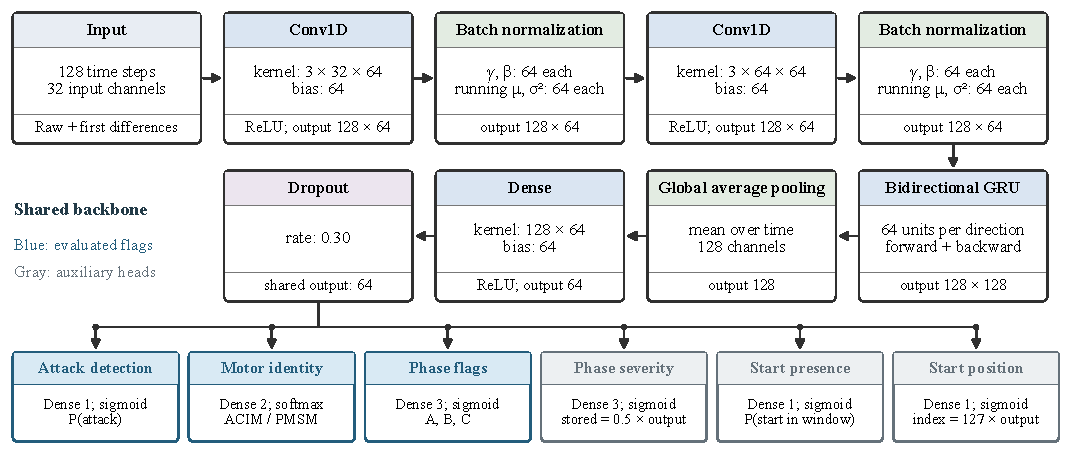
\includegraphics[width=.9\linewidth,height=.4\textheight,keepaspectratio]{figures/architecture_rebalanced_apec2027.pdf}
    \DIFaddendFL \caption{\DIFdelbeginFL \DIFdelFL{Information flow architecture detailing }\DIFdelendFL \DIFaddbeginFL \DIFaddFL{The evaluated multihead CNN--Bi-GRU. Six parallel output heads share }\DIFaddendFL the \DIFdelbeginFL \DIFdelFL{dual-stream feature engineering }\DIFdelendFL \DIFaddbeginFL \DIFaddFL{convolutional }\DIFaddendFL and \DIFdelbeginFL \DIFdelFL{preprocessing pipeline}\DIFdelendFL \DIFaddbeginFL \DIFaddFL{recurrent representation. Blue heads provide attack, motor, and phase classifications; gray heads are auxiliary severity/timing outputs}\DIFaddendFL .}
    \label{architecture}
\DIFdelbeginFL %DIFDELCMD < \end{figure}
%DIFDELCMD < %%%
\DIFdelend \DIFaddbegin \end{figure*}
\DIFaddend


Regularization is provided by Batch Normalization, dropout, \DIFdelbegin \DIFdel{early stopping based on validation PR-AUC, and a cosine learning-rate schedule}\DIFdelend \DIFaddbegin \DIFadd{and early stopping. The reported fine-tuning run uses Adam at $3\times10^{-4}$, batch size 128, gradient-norm clipping at 1, and patience 12. The learning rate is halved after five unimproved epochs, with a minimum of $10^{-5}$}\DIFaddend .

\subsection{Addressing Class Imbalance}
\DIFdelbegin \DIFdel{The merged dataset is class-imbalanced (roughly }\DIFdelend \DIFaddbegin \DIFadd{Approximately }\DIFaddend 80\% \DIFdelbegin \DIFdel{attack and 20\% normal). Rather than rebalancing through }\DIFdelend \DIFaddbegin \DIFadd{of the windows are attack-labeled. All training windows are retained without }\DIFaddend under/oversampling\DIFdelbegin \DIFdel{, the full dataset is retained and split using stratified train-test partitioning to preserve the original class proportions. Imbalance is handled during optimization via class-weighted binary }\DIFdelend \DIFaddbegin \DIFadd{. Rebalanced fine-tuning is performed with training-derived, fixed inverse-frequency attack weights: 2.5445 for normal and 0.6223 for attack. Motor identity is trained using standard two-class categorical }\DIFaddend cross-entropy\DIFdelbegin \DIFdel{, with fixed weights(\texttt{normal}=1.0, \texttt{attack}=1.5). This increases the cost of attack misclassification while preserving complete coverage of normal operating behavior}\DIFdelend \DIFaddbegin \DIFadd{: a larger loss is assigned when the correct motor receives a smaller predicted probability. Only attack windows are included, with inverse-frequency motor-class weights. For each phase, half the loss weight is assigned to affected labels, with one quarter each assigned to normal zeros and unaffected phases during attacks}\DIFaddend .

\subsection{Temporal Feature Engineering}
\DIFdelbegin \DIFdel{Early iterations used only first-order differences to emphasize signal velocity; however, this removed absolute magnitude information. The final pipeline computes first-order differences , preserves sequence length }\DIFdelend \DIFaddbegin \DIFadd{First-order differences are computed with sequence length preserved }\DIFaddend by prepending the first time step, \DIFdelbegin \DIFdel{and concatenates the differences }\DIFdelend \DIFaddbegin \DIFadd{then concatenated }\DIFaddend with the raw features. The resulting representation is feature-wise standardized, providing both absolute-state context and rate-of-change dynamics.


\DIFdelbegin \section{\DIFdel{Experimental Results and Threshold Tuning}}
%DIFAUXCMD
\addtocounter{section}{-1}%DIFAUXCMD
\DIFdelend \DIFaddbegin \subsection{\DIFadd{Multihead Loss and Evaluation Protocol}}
\DIFadd{The windows are partitioned 80/20 by stratified sampling at seed 42: 94,157 training and 23,540 evaluation windows (4,626 normal; 18,914 attack). The evaluation partition is used for checkpoint selection. Adjacent windows share 112 of 128 samples, and recordings can occur in both partitions.
}\DIFaddend

\DIFdelbegin \DIFdel{The network is
trained with Adam and }\DIFdelend \DIFaddbegin \DIFadd{A pretrained multihead checkpoint is fine-tuned for 45 epochs. The implemented objective is
}{\color{blue}\begin{equation}\underline{\displaystyle \mathcal{L}=\sum_{k\in\{a,m,p,s,o,t\}}\lambda_k\mathcal{L}_k,
 \qquad \lambda_k\equiv1,}\label{eq:multitask_loss}\end{equation}}
\DIFadd{where $a,m,p,s,o,t$ denote attack, motor, phases, severity, start presence, and start position. All six outer coefficients remain fixed; no adaptive task weighting is applied. Training-derived class weights and masks are retained within each loss, so equal coefficients do not imply equal gradient contributions.
}

\DIFadd{Weighted }\DIFaddend binary cross-entropy \DIFdelbegin \DIFdel{. Because }\DIFdelend \DIFaddbegin \DIFadd{is used for attack, phases, and start presence. Motor categorical cross-entropy is evaluated only on attack windows. For severity targets divided by 0.5, $\mathcal{L}_s=0.5\,\mathrm{MAE}_{+}+0.5\,\mathrm{MSE}_{+}+0.05\,\mathrm{MAE}_{-}$, where $+$/$-$ denote affected/unaffected phase labels. Position targets are divided by 127, and MAE is evaluated only for known starts.
}

\DIFadd{Checkpoints are selected by the mean of six task utilities: attack balanced accuracy, conditional motor balanced accuracy, phase balanced accuracy averaged over all/attack windows, start-presence F1, and two regression utilities. Each regression utility is $\max(0,\min(1,1-E/(2E_{\rm ref})))$, using MAE $E$ and the error $E_{\rm ref}$ of a training-median reference. Epoch 45 is selected.
}

\section{\DIFadd{Experimental Results}}

\DIFadd{Since }\DIFaddend cyber-attack detection prioritizes missed-attack reduction, performance is tracked using \DIFdelbegin \DIFdel{Precision, Recall, and PR-AUC rather than accuracyalone}\DIFdelend \DIFaddbegin \DIFadd{precision, recall, F1, balanced accuracy, and accuracy}\DIFaddend .

%DIF < Training uses a cosine learning-rate schedule (decaying to 10\% of the base rate) and early stopping on validation PR-AUC with best-weight restoration.
\DIFdelbegin \DIFdel{To improve the operating point beyond the default sigmoid threshold, we apply an epoch-wise threshold tuning routine that scans decision thresholds in $[0.1,0.9]$ and selects the value maximizing validation F1. With class-weighted }\DIFdelend \DIFaddbegin \DIFadd{Attack and phase outputs use the fixed threshold 0.5. With rebalanced }\DIFaddend training, dual-stream (raw+differential) inputs, and the \DIFdelbegin \DIFdel{Bi-GRU architecture, the proposed pipeline substantially outperforms the LSTM baseline and achieves $\sim$92\%test accuracy . It remains effective for low-severity attacks, achieving $\sim$96\%detection accuracy for $(0<\alpha \le 0.001)$ (}\DIFdelend \DIFaddbegin \DIFadd{CNN--Bi-GRU architecture, an accuracy of 93.46\%, balanced accuracy of 90.59\%, precision of 96.50\%, and attack recall of 95.32\% are obtained. Normal-window false positives are 14.14\%; average precision is 0.9937 and ROC-AUC is 0.9758 (area under the receiver operating characteristic curve). Detection errors are shown in Fig.~\mbox{\ref{fig:confusion_matrix}}; attack recall across stored severity groups is shown in }\DIFaddend Fig.~\mbox{\ref{fig:Severityeffect}}\DIFdelbegin \DIFdel{)}\DIFdelend .

\DIFdelbegin \DIFdel{To contextualize these results, we compare against an unoptimized LSTMbaseline and prior PMU-based \mbox{\cite{guha}} and IED-based \mbox{\cite{aljohani2024}} approaches, as summarized in Table.~\mbox{\ref{tab:comparison}}While these infrastructures can reach comparable accuracies, they require higher-cost instrumentation and are less suitable for consumer-edge deployment. In contrast, our EMU-based Bi-GRU framework provides competitive performance using low-cost sensing at the PCC.
}%DIFDELCMD < \begin{figure}
%DIFDELCMD <     \centering
%DIFDELCMD <     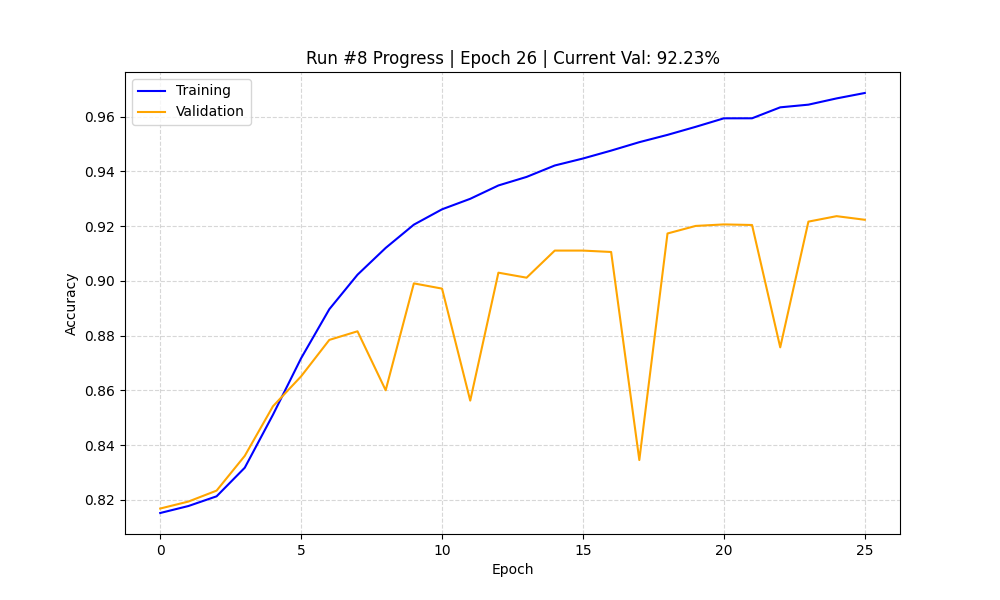
\includegraphics[width=.9\linewidth,height=.4\textheight,keepaspectratio]{image.png}
%DIFDELCMD <     %%%
%DIFDELCMD < \caption{%
{%DIFAUXCMD
\DIFdelFL{Training and Validation Accuracy over Epochs}}
    %DIFAUXCMD
%DIFDELCMD < \label{fig:placeholder}
%DIFDELCMD < \end{figure}
%DIFDELCMD < %%%
\DIFdelend \DIFaddbegin \DIFadd{The LSTM, CNN--LSTM, CNN--Bi-GRU, and proposed results are compared in Table~\mbox{\ref{tab:comparison}}. The three reference models were trained with identical inputs, partition, width 64, Adam learning rate $10^{-3}$, batch size 128, and attack-loss class weights 1.0/1.5 for at most 40 epochs. Checkpoints were selected by balanced accuracy at threshold 0.5. Additional multihead pretraining and rebalanced fine-tuning were applied to the proposed model; complete pipelines are compared, rather than isolated architecture effects.
}\DIFaddend


\DIFdelbegin \APECReviewOldTableA{}\DIFdelend \DIFaddbegin \APECReviewNewTableB{}\DIFaddend






\begin{figure}
    \centering
    \DIFdelbeginFL %DIFDELCMD < 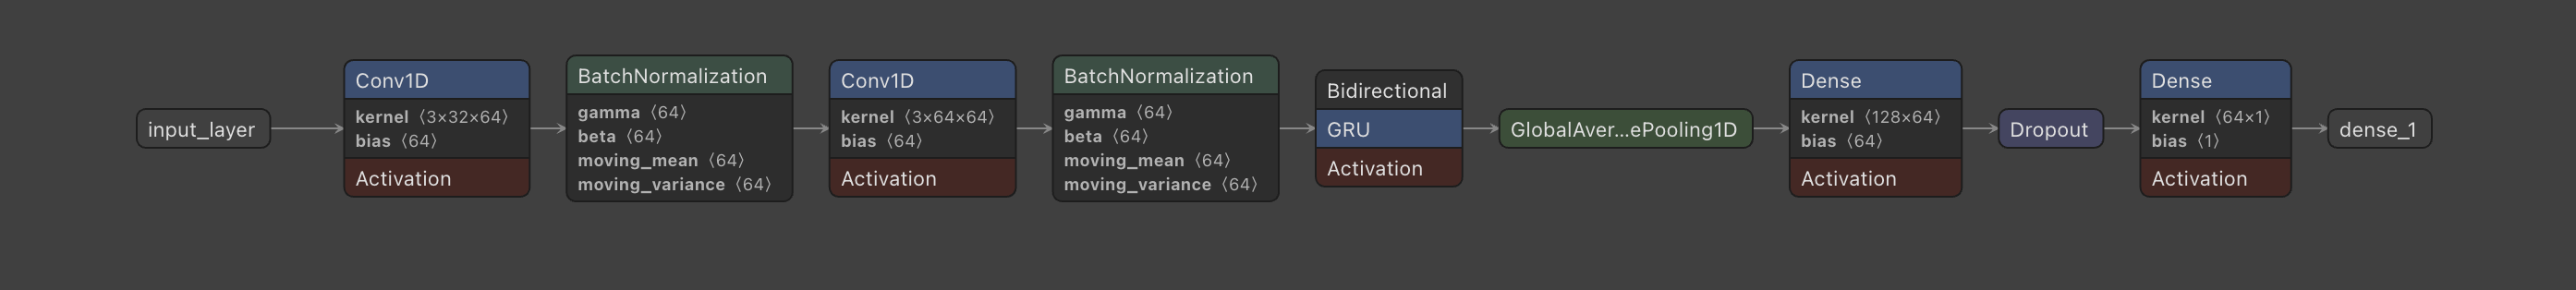
\includegraphics[width=.9\linewidth,height=.4\textheight,keepaspectratio]{Screenshot 2026-03-06 at 10.53.36 PM.png}
%DIFDELCMD <     %%%
\DIFdelendFL \DIFaddbeginFL 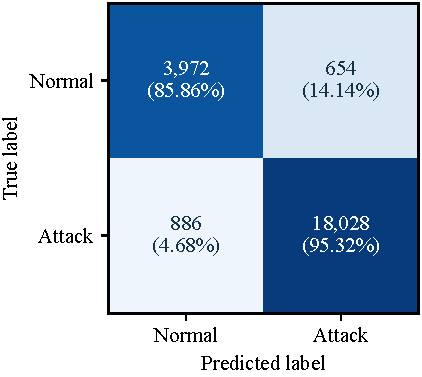
\includegraphics[width=.9\linewidth,height=.4\textheight,keepaspectratio]{figures/confusion_matrix_rebalanced_author.pdf}
    \DIFaddendFL \caption{\DIFdelbeginFL \DIFdelFL{Model Structure}\DIFdelendFL \DIFaddbeginFL \DIFaddFL{Binary FDIA detection confusion matrix at threshold 0.5.}\DIFaddendFL }
    \DIFdelbeginFL %DIFDELCMD < \label{fig:placeholder}
%DIFDELCMD < %%%
\DIFdelendFL \DIFaddbeginFL \label{fig:confusion_matrix}
\DIFaddendFL \end{figure}

\DIFdelbegin %DIFDELCMD < \clearpage
%DIFDELCMD < \begin{figure}
%DIFDELCMD <     %%%
\DIFdelendFL \DIFaddbeginFL \begin{figure}[!t]\DIFaddendFL \centering
    \DIFdelbeginFL %DIFDELCMD < 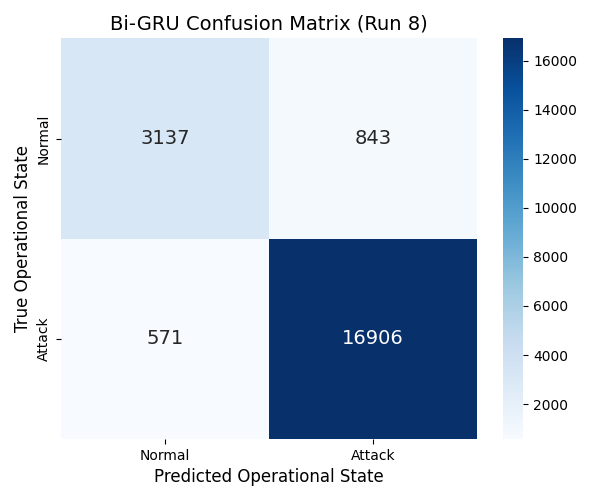
\includegraphics[width=.9\linewidth,height=.4\textheight,keepaspectratio]{Confusion}
%DIFDELCMD <     %%%
\DIFdelendFL \DIFaddbeginFL 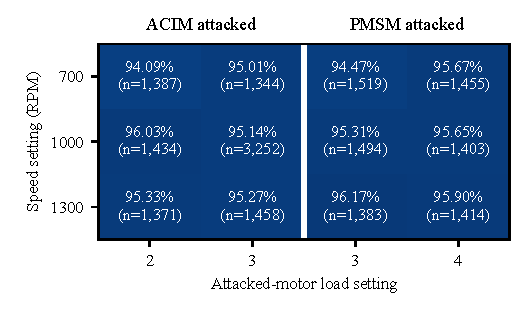
\includegraphics[width=.9\linewidth,height=.4\textheight,keepaspectratio]{figures/operating_conditions_rebalanced.pdf}
    \DIFaddendFL \caption{\DIFdelbeginFL \DIFdelFL{Confusion Matrix}\DIFdelendFL \DIFaddbeginFL \DIFaddFL{Attack recall and attack-window counts for all 12 recorded operating conditions. Both motors operate; labels identify the attacked motor's settings. Threshold 0.5 is fixed throughout.}\DIFaddendFL }
    \DIFdelbeginFL %DIFDELCMD < \label{fig:placeholder}
%DIFDELCMD < %%%
\DIFdelendFL \DIFaddbeginFL \label{fig:operating_conditions}
\DIFaddendFL \end{figure}

\DIFdelbegin %DIFDELCMD < \begin{figure}[H]
%DIFDELCMD <     %%%
\DIFdelendFL \DIFaddbeginFL \begin{figure*}[!t]
    \DIFaddendFL \centering
    \DIFdelbeginFL %DIFDELCMD < 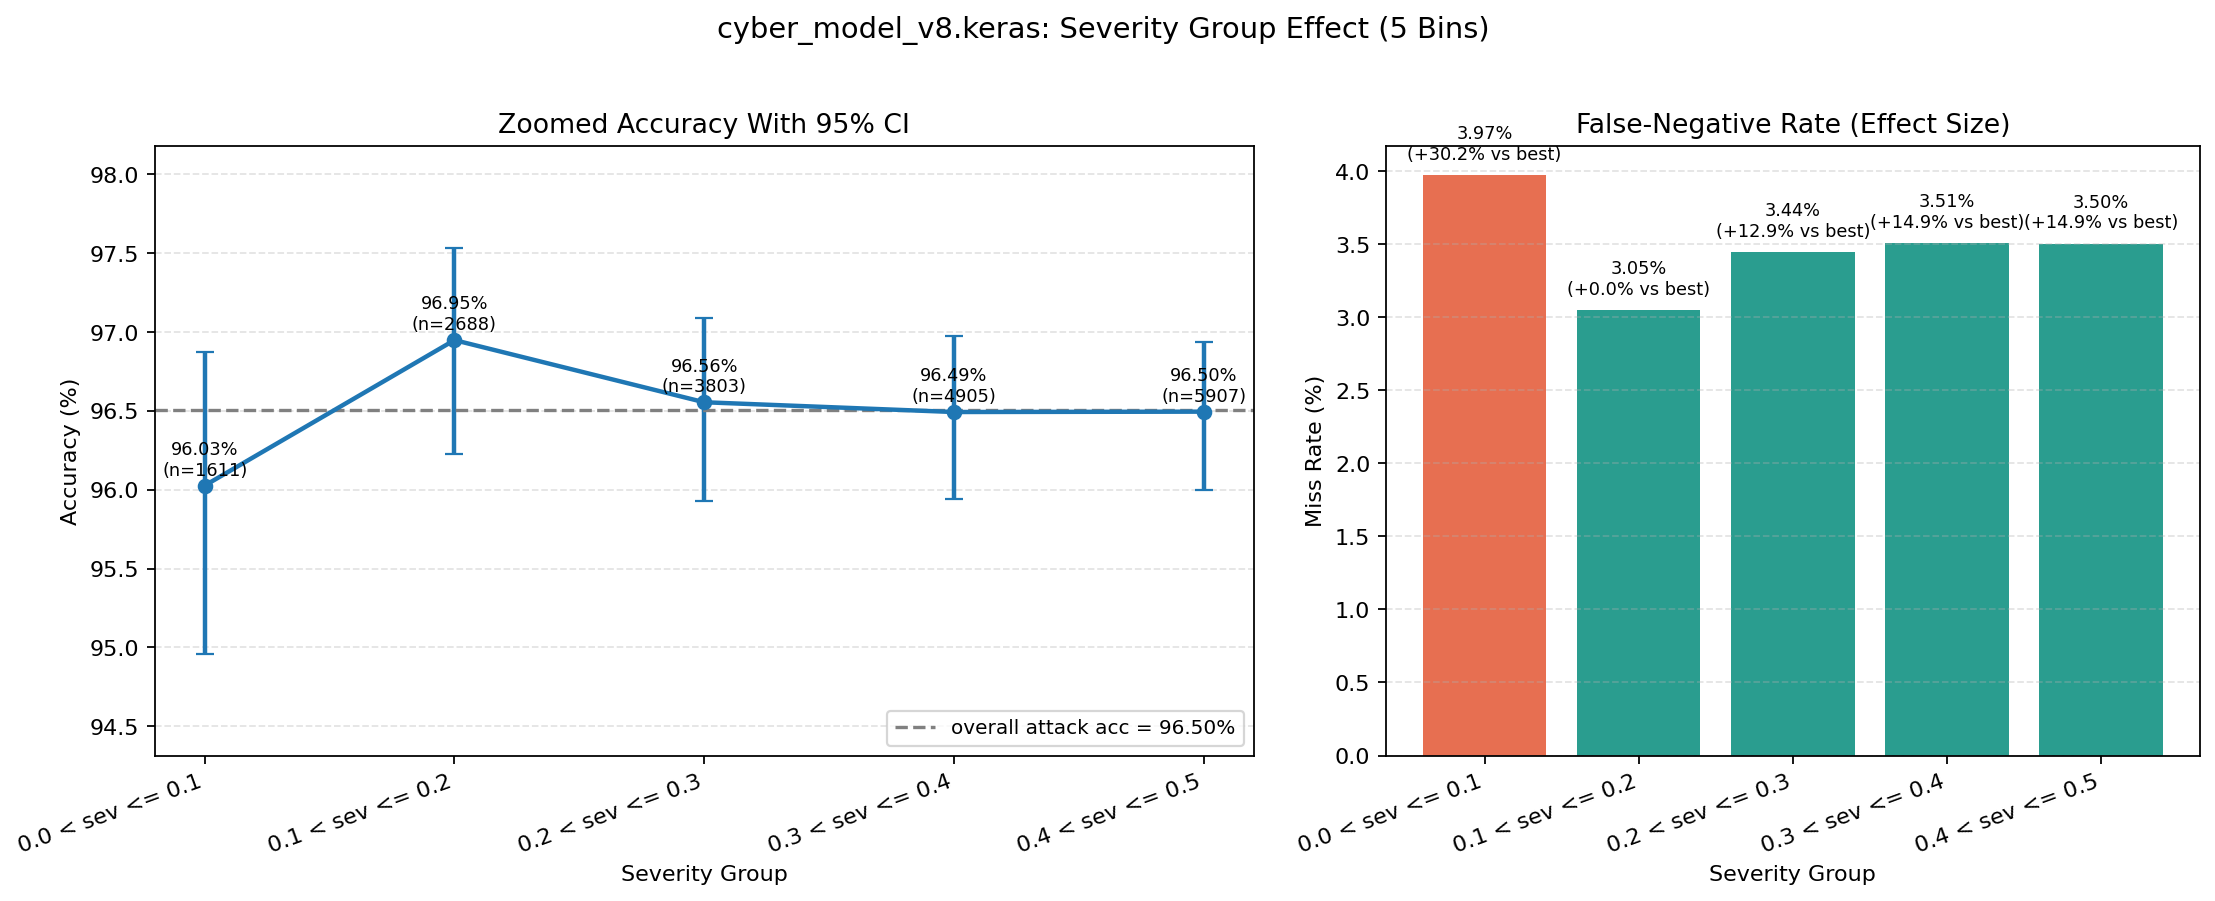
\includegraphics[width=.9\linewidth,height=.4\textheight,keepaspectratio]{figures/plot_severity_group_effect_5bins.png}
%DIFDELCMD <     %%%
\DIFdelendFL \DIFaddbeginFL 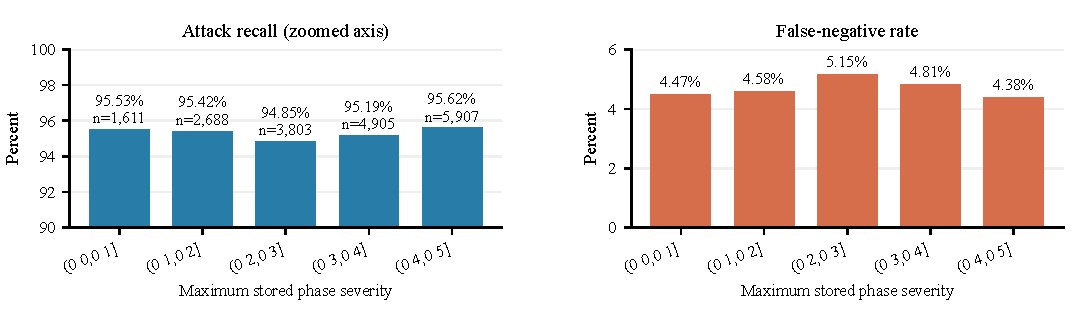
\includegraphics[width=.9\linewidth,height=.4\textheight,keepaspectratio]{figures/severity_group_recall_rebalanced.pdf}
    \DIFaddendFL \caption{\DIFdelbeginFL \DIFdelFL{Accuracy }\DIFdelendFL \DIFaddbeginFL \DIFaddFL{Attack recall }\DIFaddendFL and \DIFdelbeginFL \DIFdelFL{False Negative }\DIFdelendFL \DIFaddbeginFL \DIFaddFL{false-negative rate }\DIFaddendFL in \DIFdelbeginFL \DIFdelFL{Different Severity Groups}\DIFdelendFL \DIFaddbeginFL \DIFaddFL{stored severity groups, from the selected rebalanced model.}\DIFaddendFL }
    \label{fig:Severityeffect}
\DIFdelbeginFL %DIFDELCMD < \end{figure}
%DIFDELCMD < %%%
\DIFdelend \DIFaddbegin \end{figure*}
\DIFaddend



\DIFdelbegin \section{\DIFdel{Conclusion and Future Work}}
%DIFAUXCMD
\addtocounter{section}{-1}%DIFAUXCMD
\DIFdelend \DIFaddbegin \begin{figure*}[!t]\centering
    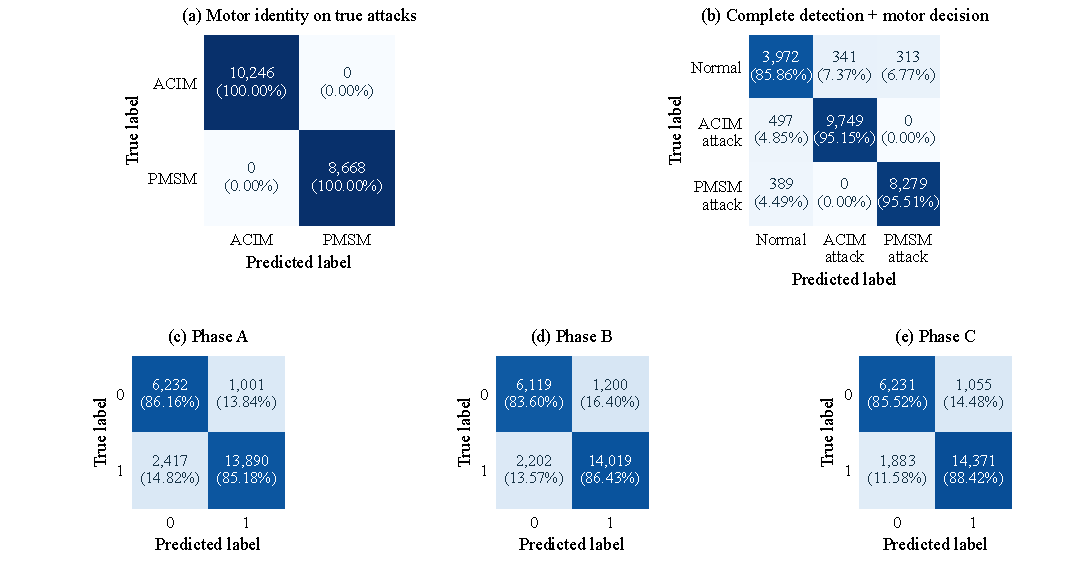
\includegraphics[width=.9\linewidth,height=.4\textheight,keepaspectratio]{figures/classification_confusion_rebalanced.pdf}
    \caption{\DIFaddFL{Motor identity conditional on true attacks, complete detection-plus-motor decisions, and raw phase A/B/C confusion matrices. Normal zero-phase labels are included in phase evaluation. Cells show counts and true-row percentages; phase 0/1 denotes unaffected/attacked.}}
    \label{fig:joint_outputs}
\end{figure*}
\DIFaddend

\DIFdelbegin \DIFdel{This work successfully demonstrates that low-cost, IoT-enabled EMU can serve as highly effective,localized sensors for cyber attack detection in AC power systems. By addressing critical data bottlenecks through class weighting and advanced feature preservation,the proposed Bidirectional GRU framework reliably processes complex 16-feature time-series data to classify operational states with high accuracy . Having established this supervised benchmark, future work will expand the framework to detect a broader range of fault and disturbance scenarios beyond cyber attacks (e.g. }\DIFdelend \DIFaddbegin \subsection{\DIFadd{Real-Time Processing Feasibility}}
\DIFadd{For the approximately 7-Hz recordings used here, an 18.29-s nominal window and 2.29-s update interval are obtained from 128 samples and stride 16. The up-to-60-Hz device capability is separate from this recording rate. Processing 1,000 validation windows (batch 1}\DIFaddend , \DIFdelbegin \DIFdel{abnormal operating conditions and component-level faults). We will also extend the PCC-based measurement strategy to function as a comprehensive observability layer, enabling unified monitoring and event classification using EMU data at the PCC}\DIFdelend \DIFaddbegin \DIFadd{50 warm-ups) on an Intel Core Ultra 9 285K CPU with four threads (TensorFlow 2.21) is completed in 4.50~ms mean, 5.19~ms 95th-percentile, and 9.26~ms maximum, including preprocessing, all six heads, and decoding. The update interval is met in every measured call, supporting real-time window processing on this host. Window duration is not attack-to-alarm delay; acquisition, communication, and event-detection delays remain unmeasured.
}


\subsection{\DIFadd{Motor and Phase Identification}}
\DIFadd{All 10,246 ACIM and 8,668 PMSM attack windows are correctly identified by the motor head when evaluated conditional on true attacks. Including detector misses, correct detection plus identity is 95.32\%, and the complete normal/ACIM/PMSM decision has 93.46\% accuracy (Fig.~\mbox{\ref{fig:joint_outputs}}). This conditional 100\% identity result is distinct from complete-pipeline performance.
}

\DIFadd{Raw phase outputs include all 23,540 windows, including normal $(0,0,0)$ labels. Exact ABC accuracy is 75.27\%, mean phase balanced accuracy is 85.88\%, and macro-F1 is 0.8965. Predicting 111 for every window gives 57.85\% exact accuracy. On normal windows, 86.10\% have all flags correctly zero. The auxiliary severity MAE is 0.1243 on affected phases, versus 0.1226 for the training-median baseline; start-presence F1 is 0.425 and known-start position MAE is 19.23 samples. These auxiliary results do not support reliable severity/timing claims.
}





\subsection{\DIFadd{Motor Identification under Common Configurations}}
\DIFadd{All 18,914 attack windows are used for the overall motor result in Table~\mbox{\ref{tab:matched_motor_settings}}. An additional control is provided by selecting only speed, load, phase-flag, and stored phase-severity tuples represented for both attacked motors. Of the attack windows, 8,841 satisfy this matching rule, spanning 596 shared tuples; the remaining 10,073 are retained in the overall result but excluded from this subset. Thus, 8,841 is a controlled subset, not the total attack cohort.
}

\APECReviewNewTableC{}



\DIFadd{For the shared settings, conditional identity is 100\% and detection plus identity is 95.28\%. Identification from aggregate PCC features is therefore supported even when the recorded settings match between motor classes. Joint errors are caused by detector misses. The original evaluation windows are reused; no additional recording holdout is introduced.
}

\subsection{\DIFadd{Coverage of Recorded Operating Conditions}}
\DIFadd{Across all 12 recorded motor--speed--load combinations, recall ranges from 94.09\% (ACIM, 700 RPM, load setting 2) to 96.17\% (PMSM, 1300 RPM, load setting 3), at the same threshold 0.5 (Fig.~\mbox{\ref{fig:operating_conditions}}). This supports consistent attack sensitivity across represented settings.
}



\section{\DIFadd{Conclusion and Future Work}}

\DIFadd{FDIA detection and attacked-motor identification have been demonstrated from aggregate PCC measurements while both motors operate. Identification is supported across matching recorded settings, and consistent sensitivity is obtained across the represented speeds and loads. The fixed-weight multihead CNN--Bi-GRU can be processed within the measurement-update interval on the benchmarked CPU. The framework will be extended to benign transients and other faults, with additional motor counts and independent recordings evaluated before broader deployment.
}

\DIFadd{Results use overlapping-window validation, with no independent recording test. Performance with ten motors remains unestablished and requires dedicated validation.
}

\section*{\DIFadd{Acknowledgment}}
\DIFadd{OpenAI Codex assisted with manuscript revisions, evaluation code, and diagnostic figures. Reported metrics were computed from the recorded dataset}\DIFaddend .

\bibliographystyle{IEEEtran}
\DIFdelbegin %DIFDELCMD < \bibliography{IEEEabrv,bibliography}
%DIFDELCMD < %%%
\DIFdelend \DIFaddbegin \bibliography{References_main}
\DIFaddend

\end{document}
